% !TEX root =main.tex


\section{Definition of Multi-party PSI with Fair Compensation}\label{sec::F-PSI-model}%\label{Fair-PSI-Protocol}





In this section, we present the notion of multi-party PSI with Fair Compensation  (\p) which allows either all clients to get the result or the honest parties to be financially compensated if the protocol aborts in an unfair manner, where only dishonest parties learn the result.  


%We first provide the security model and assumptions used in \p. After that, we provide three subprotocols utilised by a construction, called \withFai (\fpsi), that realises \p; namely, \vopr, \zspa, and its extension \zspaa.  After that, we will give an overview of \fpsi followed by \fpsi's detailed description. 


 
 
 
 
 
 
 
% \subsection{The Model} In this section, we provide the security model of our protocol. In F-PSI, three types of parties are involved; namely, (1) a set of clients $\{A_{\st 1},...,A_{\st m}\}$ potentially \emph{malicious} (i.e., active adversaries) and all but one may collude with each other, (2) a non- colluding dealer, client D, potentially semi-honest (i.e., a passive adversary), and (3) an auditor $Aud$ potentially semi-honest, where all parties except the auditor have input set. For simplicity, we assume that given an address one can determine whether it belongs to an auditor. The basic functionality that a multi-party PSI  computes is defined as $f^{\st\text{PSI}} (S_{\st 1},..., S_{\st m+1})\rightarrow\underbrace{(S_{\st\cap},..., S_{\st\cap})}_{\st m+1}$, where $S_{\st\cap}=S_{\st 1} \cap, ..., \cap S_{\st m+1}$.  To formally define the \emph{fair PSI with compensations}, and add the fairness guarantee, we equip the above PSI functionality with the following predicate triple,  $Q:=(Q^{\st \text{Init}}, Q^{\st \text{Del}}, Q^{\st \text{Abt}})$  that are invoked before functionality $f^{\st \text{PSI}}$ is executed. These predicates were initially proposed in \cite{KiayiasZZ16}; nevertheless, below we will provide more formal accurate definition of them. First, we present a high level description of  these predicates. Predicate $Q^{\st \text{Init}}$ specifies under which condition the protocol should start executing (i.e., when all set owners have enough deposit), $Q^{\st \text{Del}}$ determines the situation where parties receive their output (i.e., when  honest parties receive their deposit back) while $Q^{\st \text{Abt}}$ specifies under which circumstance the simulator can force parties to abort (i.e., when an honest party receives its deposit back plus a predefined amount of compensation). Intuitively, by requiring a fair PSI protocol to implement such a wrapped version of $f^{\st\text{PSI}}$ that includes $Q$, we will ensure that an honest set owner might only abort if $Q^{\st \text{Abt}}$ returns  $1$, and might output a valid value if $Q^{\st \text{Del}}$ returns $1$. Now, we formally define each of these predicates.  
 
 
 
  %\subsection{The Model}\label{sec::F-PSI-model}
  
  
In a  $\mathcal{PSI}^{\st \mathcal{MFC}}$, three types of parties are involved; namely, (1) a set of clients $\{A_{\st 1},...,A_{\st m}\}$ potentially \emph{malicious} (i.e., active adversaries) and all but one may collude with each other, (2) a non-colluding dealer, $D$, potentially semi-honest (i.e., a passive adversary) and has an input set, and (3) an auditor \aud potentially semi-honest, where all parties except \aud have input set. For simplicity, we assume that given an address one can determine whether it belongs to \aud. 


The basic functionality that any multi-party PSI computes can be defined as $f^{\st\text{PSI}} (S_{\st 1},..., S_{\st m+1})\rightarrow\underbrace{(S_{\st\cap},..., S_{\st\cap})}_{\st m+1}$, where $S_{\st\cap}= S_{\st 1} \cap S_{\st 2}, ...,\cap\  S_{\st m+1}$.  To formally define a \p, we equip the above PSI functionality with four predicates,  $Q:=(\qinit, \qdel, \qUnFAbt, \qFAbt)$, which ensure that certain financial conditions are met. 
   %  that are invoked after the functionality $f^{\st \text{PSI}}$ is executed. 
   We borrow three of these predicates (i.e., $\qinit, \qdel, \qUnFAbt$) from the ``fair and robust multi-party computation'' initially proposed in \cite{KiayiasZZ16}; nevertheless, we will (i) introduce an additional predicate  \qFAbt and (ii) provide more formal accurate definitions of these predicates. 
   
Predicate \qinit specifies under which condition a protocol that realises \p should start executing, i.e., when all set owners have enough deposit. Predicate \qdel determines in which situation parties receive their output, i.e., when honest parties receive their deposit back. Predicate \qUnFAbt specifies under which condition the simulator can force parties to abort if the adversary learns the output,  i.e., when an honest party receives its deposit back plus a predefined amount of compensation. Predicate \qFAbt specifies under which condition the simulator can force parties to abort if the adversary receives no output, i.e., when honest parties receive their deposits back. We observed that the latter predicate should have been defined in the generic framework in \cite{KiayiasZZ16} too; as the framework should have also captured the cases where an adversary may abort without learning any output after the onset of the protocol.  Intuitively, by requiring any protocol that realises \p to implement a wrapped version of $f^{\st\text{PSI}}$ that includes $Q$, we will ensure that an honest set owner only aborts in an unfair manner if \qUnFAbt returns  $1$, it only aborts in a fair manner if \qFAbt returns  $1$, and outputs a valid value if \qdel returns $1$. Now, we formally define each of these predicates.  
 

 
 
 \begin{definition}
 %
  [\qinit: Initiation predicate] Let $\mathcal{G}$ be a stable ledger, $adr_{\st sc}$ be smart contract $sc$'s address, $Adr$ be a set of $m+1$ distinct addresses, and $\xc$ be a fixed amount of coins. Then, predicate $\qinit(\mathcal{G}, adr_{\st sc}, m+1, Adr, \xc)$ returns $1$ if every address in $Adr$ has at least $\xc$ coins in $sc$; otherwise, it returns $0$. 
 %
 \end{definition}

 
 
    \begin{definition}  [\qdel:
    %
    Delivery predicate] Let $pram:=(\mathcal{G}, adr_{\st sc}, \xc)$ be the parameters defined above, and   $adr_{\st i}\in Adr$ be the address of an honest party. 
    %
%    Let also $G$ be a compensation function that takes as input  two parameters $(deps, m')$, where $deps$ is the amount of coins  that all $m+1$ parties  deposit; it returns the amount of compensation each honest party must receive, i.e., $G(deps, m')\rightarrow c'$. 
    %
    Then, predicate $\qdel(pram, adr_{\st i})$ returns $1$ if $adr_{\st i}$ has sent $\xc$ amount to $sc$ and received  $\xc$ amount from it; thus,  its balance in $sc$ is $0$. Otherwise, it returns $0$. 
 %
  \end{definition}
 
 
 
   \begin{definition}  [\qUnFAbt: UnFair-Abort predicate]
   %
 Let $pram:=(\mathcal{G}, adr_{\st sc}, \xc)$ be the parameters defined above, and $Adr'\subset Adr$ be a set containing honest parties' addresses, $m' = |Adr'|$,  and   $adr_{\st i}\in Adr'$. Let also $G$ be a compensation function that takes as input  three parameters $(\depsc, adr_{\st i}, m')$, where $\depsc$ is the amount of coins  that all $m+1$ parties  deposit. It returns the amount of compensation each honest party must receive, i.e., $G(\depsc, ard_{\st i}, m')\rightarrow \xci$. Then, predicate $Q^{\st \text{UnF-Abt}}$ is defined as $\qUnFAbt(pram, G, \depsc, m', adr_{\st i})\rightarrow (a,b)$, where $a=1$ if $adr_{\st i}$ is an honest party's address and $adr_{\st i}$ has sent $\xc$ amount to $sc$ and received  $\xc+\xci$  from it, and $b=1$ if $adr_{\st i}$ is \aud's address and $adr_{\st i}$ received $\xci$  from $sc$. Otherwise, $a=b=0$. 
  %
  \end{definition}
  
  
\begin{definition}  [\qFAbt: Fair-Abort predicate]
   %
 Let $pram:=(\mathcal{G}, adr_{\st sc}, \xc)$ be the parameters defined above, and $Adr'\subset Adr$ be a set containing honest parties' addresses, $m' = |Adr'|$,     $adr_{\st i}\in Adr'$, and  $adr_{\st j}$ be \aud's address. Let $G$ be the compensation function, defined above and let $G(deps, ard_{\st j}, m')\rightarrow \xc_{\st j}$ be the compensation that the auditor must receive.  Then, predicate $\qFAbt(pram, G, \depsc, m', adr_{\st i}, adr_{\st j})$ returns $1$, if $adr_{\st i}$ (s.t. $adr_{\st i}\neq adr_{\st j}$) has sent $\xc$ amount to $sc$ and received  $\xc$  from it, and $adr_{\st j}$ received $\xc_{\st j}$  from $sc$. Otherwise, it returns $0$. 
  %
 \end{definition}
  
  
  
 
 Next, we present a formal definition of \p. %Note that we have upgraded the simulation-based definition of secure computation (i.e., Definition \ref{def::MPC-active-adv}) to define the security requirements of \p, by incorporating the above predicates into the definition. 
 
\begin{definition}[\p]\label{def::PSI-Q-fair}
Let $f^{\st \text{PSI}}$ be the multi-party PSI functionality defined above. We say  protocol $\Gamma$ realises  $f^{\st \text{PSI}}$ with $Q$-fairness in the presence of $m-1$ static active-adversary clients (i.e., $A_{\st j}$s) or a static passive dealer $D$ or passive auditor $Aud$, if for every non-uniform probabilistic polynomial time adversary $\mathcal{A}$ for the real model, there exists a non-uniform probabilistic polynomial-time adversary (or simulator) $\mathsf{Sim}$ for the ideal model, such that for every $I\in \{A_{\st 1},...,A_{\st m}, D, Aud\}$, it holds that: 

\begin{equation*}
\{\mathsf {Ideal}^{\st \mathcal{W}(f^{\st \text{PSI}},Q)}_{\st \mathsf{Sim}(z), I}(S_{\st 1},..., S_{\st m+1})\}_{\st S_{\st 1},..., S_{\st m+1},z}\stackrel{c}{\equiv} \{\mathsf{Real}_{\st \mathcal{A}(z), I}^{\st \Gamma}(S_{\st 1},..., S_{\st m+1}) \}_{\st S_{\st 1},..., S_{\st m+1},z}
\end{equation*}
where  $z$ is an auxiliary input given to $\mathcal{A}$ and  $\mathcal{W}(f^{\st \text{PSI}},Q)$ is a functionality that wraps $f^{\st \text{PSI}}$ with predicates $Q:=(\qinit, \qdel, \qUnFAbt, \qFAbt)$. 
  \end{definition}
 
%   \begin{definition}  [$Q^{\st \text{Del}}$:
%   %
%    Delivery predicate] Let $pram:=(\mathcal{G}, adr_{\st sc}, c)$ be the parameters defined above, and   $adr_{\st i}\in Adr$ be the address of an honest party. Let also $G$ be a compensation function that takes as input  two parameters $(deps, m')$, where $deps$ is the amount of coins  that all $m+1$ parties  deposit; it returns the amount of compensation each honest party must receive, i.e., $G(deps, m')\rightarrow c'$. Then, predicate $Q^{\st \text{Del}}(pram, G, deps, m', adr_{\st i})$ returns $1$ if $adr_{\st i}$ has sent $c$ amount to $sc$ and received  $c+c'$  from it. Otherwise, it returns $0$. 
% %
%  \end{definition}
 
 
 
%  \begin{definition}  [$Q^{\st \text{Abt}}$: Abort predicate]
% Let $pram:=(\mathcal{G}, adr_{\st sc}, c)$ be the parameters defined above, and $Adr'\subset Adr$ be a set containing honest parties' addresses, $m' = |Adr'|$,  and   $adr_{\st i}\in Adr'$. Let also $G$ be a compensation function that takes as input  three parameters $(deps, adr_{\st i}, m')$, where $deps$ is the amount of coins  that all $m+1$ parties  deposit, $adr_{\st i}$ is an hones party's address, and $m' = |Adr'|$; it returns the amount of compensation each honest party must receive, i.e., $G(deps, ard_{\st i}, m')\rightarrow c_{\st i}$. Then, predicate $Q^{\st \text{Abt}}(pram, G, deps, m', adr_{\st i})$ returns $1$ if $adr_{\st i}$ has sent $c$ amount to $sc$ and received  $c+c'$  from it. Otherwise, it returns $0$. 
%  
%  \end{definition}
 
 %Recall, the standard simulation-based model (presented in Section \ref{}) can adequately capture the security definition of secure multi-party computation and accordingly regular PSI; however, it is not 
 

 

  
% !TEX root =main.tex


\vspace{-3mm}



\section{Other Subroutines Used in \withFai}\label{sec::subroutines}
\vspace{-1mm}

In this section, we present three subroutines and a primitive that we developed and are used in the instantiation of \p, i.e., \withFai. 


\vspace{-3mm}
\subsection{Verifiable Oblivious Polynomial Randomisation (\vopr)}\label{sec::vopr}
\vspace{-1mm}

%In this section, we present ``Verifiable Oblivious Polynomial Randomisation'' (VOPR) protocol. 

In the \vopr, two parties are involved, (i) a sender which is potentially a passive adversary and (ii) a receiver that is potentially an active adversary. The protocol allows the receiver with input polynomial $\bm\beta$ (of degree $e'$) and the sender with input random polynomials $\bm\psi$ (of degree $e$) and  $\bm{\alpha}$ (of degree $e+e'$)   to compute: $\bm\theta=\bm\psi\cdot \bm\beta+\bm\alpha$, such that (a) the receiver learns only $\bm\theta$ and nothing about the sender's input even if it sets $\bm \beta=0$, (b) the sender learns nothing, and (c) the receiver's misbehaviour is detected in the protocol. Thus, the functionality that  \vopr computes is defined as $f^{\st {\vopr}}( (\bm\psi, \bm{\alpha}), \bm\beta)\rightarrow(\bot, \bm\psi\cdot \bm\beta+\bm\alpha)$. 
%
We will use {\vopr} in \withFai for two main reasons:  (a) to let a party re-randomise its counterparty's polynomial (representing its set) and (b) to impose a MAC-like structure to the randomised polynomial; such a structure will allow a verifier to detect if \vopr's output has been modified. 

Now, we outline how we design \vopr without using any (expensive) zero-knowledge proofs.\footnote{Previously, Ghosh \textit{et al.}  \cite{GhoshN19} designed a protocol called Oblivious Polynomial Addition (OPA) to meet similar security requirements that we laid out above. But, as shown in \cite{AbadiMZ21}, OPA  is susceptible to several serious attacks. } In the setup phase, both parties represent their input polynomials in the regular coefficient form; therefore, the sender's polynomials are defined as $\bm\psi=\sum\limits^{\st e}_{\st i=0}g_{\st i}\cdot x^{\st i}$ and  $\bm\alpha=\sum\limits^{\st e+e'}_{\st j=0}a_{\st j}\cdot x^{\st j}$ and the receiver's polynomial is defined as $\bm\beta=\sum\limits^{\st e'}_{\st i=0}b_{\st i}\cdot x^{\st i}$, where $b_{\st i}\neq 0$. However, the sender computes each coefficient $a_{\st j}$ (of polynomial $\bm \alpha$) as follows,  $a_{\st j}=\sum\limits^{\substack{\st k=e'\\ \st t=e}}_{\st t,k=0} a_{\st t,k}$,  where  $t+k=j$ and each $a_{\st t,k}$ is a random value. For instance, if $e=4$ and $e'=3$, then $a_{\st 3}=a_{\st \st 0,3}+a_{\st 3,0}+a_{\st 1,2}+a_{\st 2,1}$. Shortly, we explain why polynomial $\bm\alpha$ is constructed this way. 



In the computation phase,  to compute polynomial $\bm\theta$, the two parties interactively multiply and add the related coefficients in a secure way using $\ole^{\st +}$ (presented in Section \ref{sec::OLE-plus}). Specifically,
%
%For simplicity, let $i=0$. 
%
for every $j$  (where $0\leq j\leq e'$) the sender sends $g_{\st i}$ and $a_{\st i,j}$ to an instance of  $\ole^{\st +}$, while the receiver sends $b_{\st j}$ to the same instance,  which returns $c_{\st i,j}=g_{\st i}\cdot b_{\st j}+ a_{\st i,j}$ to the receiver. This process is repeated for every $i$, where $0 \leq i \leq e$. Then, the receiver uses $c_{\st i,j}$ values to construct the resulting polynomial, $\bm\theta=\bm\psi\cdot \bm\beta+\bm\alpha$.  


The reason that the sender imposes the above structure to (the coefficients of)  $\bm\alpha$ in the setup, is to let the parties securely compute $\bm\theta$ via  $\ole^{\st +}$. Specifically, by imposing this structure (1) the sender  can blind each product $g_{\st i}\cdot b_{\st j}$  with  random value $a_{\st i,j}$ which is a component of $\bm\alpha$'s coefficient and (2) the receiver can construct a result polynomial of the form $\bm\theta=\bm\psi\cdot \bm\beta+\bm\alpha$. 


To check the result's correctness, the sender picks and sends a random value $z$ to the receiver which computes  $\bm\theta(z)$ and $\bm\beta(z)$ and sends these two values  to the sender. The sender computes  $\bm\psi(z)$ and $\bm\alpha(z)$ and then checks if equation  $\bm\theta({ z})=\bm\psi({ z})\cdot \bm\beta({ z})+\bm\alpha({ z})$ holds. It accepts the result if the check passes.   

Figure \ref{fig:VOPR} describes \vopr in detail. Note, \vopr requires the sender to insert non-zero coefficients, i.e., $b_{\st i}\neq 0$ for all $i,0 \leq i \leq e'$. If the   sender inserts a zero-coefficient, then it will learn only a random value (due to  $\ole^{\st +}$), accordingly it cannot pass \vopr's verification phase. However, such a requirement will not affect Justitia's correctness, as we will discuss in Section \ref{Fair-PSI-Protocol} and Appendix \ref{sec::error-prob}.  

\vspace{-2mm}

% !TEX root =main.tex



%%%%%%%%
\begin{figure}[!htb]%[!htbp]
\setlength{\fboxsep}{.8pt}
\begin{center}
\scalebox{.85}{
    \begin{tcolorbox}[enhanced,width=5.5in, 
    drop fuzzy shadow southwest,
    colframe=black,colback=white]
%%%%%%%%

\svs
\begin{enumerate}[leftmargin=1mm]
\small{
\item[$\bullet$] \textit{Input.}
\begin{enumerate}[leftmargin=3mm]
\item[$\bullet$]  \textit{Public Parameters}: upper bound on input polynomials' degree: $e$ and $e'$. %, where $e\geq e'$.
%\item[$\bullet$]  \textit{Sender}: picks an upper bound on input polynomials's degree:  $d$ and $d'$. It sends them to the receiver.
\item[$\bullet$]  \textit{Sender Input}:  random polynomials: $\bm\psi=\sum\limits^{\st e}_{\st i=0}g_{\st i}\cdot x^{\st i}$ and  $\bm\alpha=\sum\limits^{\st e+e'}_{\st j=0}a_{\st j}\cdot x^{\st j}$, where $g_{\st i}\stackrel{\st \$}\leftarrow \mathbb{F}_p$.  Each $a_{\st j}$ has the  form: $a_{\st j}=\sum\limits^{\substack{\st k=e'\\ \st t=e}}_{\st t,k=0} a_{\st t,k}$,  such that $t+k=j$ and $a_{\st t,k}\stackrel{\st \$}\leftarrow \mathbb{F}_p$.

\item[$\bullet$] \textit{Receiver Input}:  polynomial $\bm\beta=\bm\beta_{\st 1}\cdot \bm\beta_{\st 2}=\sum\limits^{\st e'}_{\st i=0}b_{\st i}\cdot x^{\st i}$, where $\bm\beta_{\st 1}$ is a random polynomial of degree $1$ and $\bm\beta_{\st 2}$ is an arbitrary polynomial of degree $e'-1$.


\end{enumerate}
\item[$\bullet$] \textit{Output.} The receiver gets $\bm\theta=\bm\psi\cdot \bm\beta+\bm\alpha$.
\item \textbf{Computation:}

\begin{enumerate} [leftmargin=3mm]

\item Sender and receiver together for every $j$, $0\leq j\leq e'$,  invoke $e+1$ instances of $\ole^{\st +}$. In particular, $\forall j, 0\leq j\leq e'$: sender sends $g_{\st i}$ and $a_{\st i,j}$ while the receiver sends $b_{\st j}$ to $\ole^{\st +}$ that returns: $c_{\st i,j}=g_{\st i}\cdot b_{\st j}+ a_{\st i,j}$ to the receiver ($\forall i, 0\leq i\leq e$). 


 \item The receiver sums component-wise values $c_{\st i,j}$  that results in polynomial:
 %
 \vspace{-2mm}
 %
  $$\bm\theta=\bm\psi\cdot \bm\beta+\bm\alpha=\sum\limits^{\substack{\st i=e\\ \st j=e'}}_{\st i,j=0}c_{\st i, j}\cdot x^{\st i+j}$$ 
 %
  \vspace{-2mm}
  %
 




% \item The receiver sums component-wise values $c_{\st i,j}$  that results polynomial $\bm\theta=\bm\psi\cdot \bm\beta+\bm\alpha=\sum\limits^{\st e+e'}_{\st j=0}c_{\st j}\cdot x^{\st j}$, where  each $c_{\st j}$ has   form: $c_{\st j}=\sum\limits^{\substack{\st k=e'\\ \st t=e}}_{\st  t,k=0} c_{\st t,k}$, such that $ t+k=j$.
%\item Sender: $\forall j, 1\leq j\leq 2d+1$, computes $a_{\st j}=a(x_{\st j})$ and $r_{\st j}=r(x_{\st j})$. Then, it  inserts $(a_{\st j}, r_{\st j})$ into  $\mathcal{F}_{\st OLE^{\st +}}$
%\item\label{computing-receiver} Receiver:  $\forall j, 1 \leq j\leq 2d+1$, computes $b_{\st j}=b(x_{\st j})$. Then, it  inserts $b_{\st j}$ into  $\mathcal{F}_{\st OLE^{\st +}}$ and receives $s_{\st j}=a_{\st j}+b_{\st j}\cdot r_{\st j}$. It interpolates a polynomial $s(x)$ using pairs $s_{\st j},x_{\st j}$. 
\end{enumerate}
\vs
\item \label{Verification} \textbf{Verification:}
\begin{enumerate}[leftmargin=3mm]

\item \label{picking-random-x}Sender: picks a random value  $z$ and sends it to the receiver. 


\item\label{receiver-OLE-invocation} Receiver: sends $\theta_{\st z}=\bm\theta(z)$ and $\beta_{\st z}=\bm\beta(z)$ to the sender.

\item\label{receiver-OLE-invocation} Sender:  computes $\psi_{\st z}=\bm\psi(z)$ and $\alpha_{\st z}=\bm\alpha(z)$ and checks   if equation  $\theta_{\st z}=\psi{\st z}\cdot \beta_{\st z}+\alpha_{\st z}$ holds. If the equation holds, it concludes that the computation was performed correctly. Otherwise, it aborts. 
%
\vs
\end{enumerate}
}
 \end{enumerate}
 \end{tcolorbox}
 }
\end{center}
\vs
\vs
\caption{Verifiable Oblivious Polynomial Randomization ({\vopr}) } 
\label{fig:VOPR}
\end{figure}
 %%%%%%%

%\vspace{-1mm}
\begin{theorem}\label{theorem::VOPR}
%
Let $f^{\st \vopr}$ be the functionality defined above. If the enhanced \ole (i.e., $\ole^{\st +}$) is secure against malicious (or active) adversaries, then the  Verifiable Oblivious Polynomial Randomisation (\vopr), presented in Figure \ref{fig:VOPR}, securely computes $f^{\st \vopr}$ in the presence of (i) semi-honest sender and honest receiver or (ii) malicious receiver and honest sender. 
%
\end{theorem}

\vspace{-1mm}
We refer readers to Appendix \ref{sec::proof-of-vopr} for the proof of Theorem \ref{theorem::VOPR}. 


% !TEX root =main.tex

\subsection{Zero-sum Pseudorandom Values Agreement Protocol (\zspa)}

The \zspa  allows $m$ parties (the majority of which is potentially malicious) to efficiently agree on (a set of vectors, where each $i$-th vector has) $m$ pseudorandom values such that their sum equals zero. At a high level, the parties first sign a smart contract, register their accounts/addresses in it, and then run a  coin-tossing protocol \ct to agree on a key: $k$.  Next, one of the parties generates $m-1$ pseudorandom values $z_{\scriptscriptstyle i, j}$ (where $1\leq j\leq m-1$) using key $k$ and $\mathtt{PRF}$. It sets the last value as the additive inverse of the sum of the values generated, i.e. $z_{\scriptscriptstyle i, m}=-\sum\limits^{\scriptscriptstyle m-1}_{\scriptscriptstyle j=1}z_{\scriptscriptstyle i, j}$ (similar to the standard XOR-based secret sharing \cite{Schneier0078909}). 
%
%Next, it commits to each value, where it uses $k_{\scriptscriptstyle 2}$ to generate the randomness of each commitment. 
%
Then, it constructs a Merkel tree on top of the pseudorandom values and stores only the tree's root $g$ and the key's hash value $q$ in the smart contract.  Then, each party (using the key) locally checks if the values (on the contract) have been constructed correctly; if so, then it sends a (signed) ``approved" message to the contract which only accepts messages from registered parties. Hence, the functionality that \zspa computes is defined as $f^{\st \zspa}\underbrace{(\bot,..., \bot)}_{\st m}\rightarrow \underbrace{((k, g, q),..., (k, g,q))}_{\st m}$, where $g$ is the Markle tree's root built on the pseudorandom values $z_{\st i, j}$, $q$ is the hash value of the key used to generate the pseudorandom values, and $m\geq 2$. Figure \ref{fig:ZSPA} presents \zspa in detail.  


Briefly, \zspa will be used in \withFai to allow clients $\{A_{\st 1},...,A_{\st m}\}$ to provably agree on a set of pseudorandom values, where each set represents a pseudorandom polynomial (as the elements of the set are considered the polynomial's coefficients). Due to \zspa's property, the sum of these polynomials is zero.  Each of these polynomials will be used by a client to blind/encrypt the messages it sends to the smart contract, to protect the privacy of the plaintext message (from \aud, D, and the public). To compute the sum of the plaintext messages, one can easily sum the blinded messages, which removes the blinding polynomials. 

% !TEX root =main.tex




\begin{figure}[ht]%[!htbp]
\setlength{\fboxsep}{1pt}
\begin{center}
\scalebox{.85}{
    \begin{tcolorbox}[enhanced,width=5.5in, 
    drop fuzzy shadow southwest,
    colframe=black,colback=white]


\small{

\begin{enumerate}[leftmargin=1mm]
\item[$\bullet$]    {Parties.} A set of clients $\{    A_{\st 1},...,  A_{\st m}\}$.
%
\item[$\bullet$]    {Input.}  $m$: the total number of participants, $adr$: a deployed smart contract's address, and $b$: the total number of vectors. Let $b'=b-1$. 
%
\item[$\bullet$]   {Output.}  $k$: a secret key that generates $b$ vectors $[z_{\scriptscriptstyle 0,1},...,z_{\scriptscriptstyle 0,m}],...,[z_{\scriptscriptstyle b',1},...,z_{\scriptscriptstyle b',m}]$ of pseudorandom values, $h$: hash of the key,  $g$: a Merkle tree's root, and a vector of signed messages. 


%, such that the sum of each vector's elements equals zero: $\sum\limits^{\scriptscriptstyle m}_{\scriptscriptstyle j=1}z_{\scriptscriptstyle i,j}=0$. 


\item {\textbf{Coin-tossing.} $\ct (in_{\st 1},..., in_{\st m})\rightarrow k$}. 

All participants run a coin-tossing protocol to agree on $\mathtt{PRF}$'s key, $k$.
\item\label{ZSPA:val-gen}  {\textbf{Encoding.} $\mathtt{Encode}(k, m)\rightarrow (g,q)$}.

 One of the parties takes the following steps:  
\begin{enumerate}

\item for every $i$ (where $0\leq i \leq b'$), generates $m$ pseudorandom values as follows. 
%
 $$\forall j, 1\leq j \leq m-1: z_{\scriptscriptstyle i,j}=\mathtt{PRF}(k,i||j), \hspace{5mm} z_{\scriptscriptstyle i,m}=-\sum\limits^{\scriptscriptstyle m-1}_{\scriptscriptstyle j=1}z_{\scriptscriptstyle i,j}$$
%
\vs
\item   constructs a Merkel tree on top of all pseudorandom values,  $\mkgen(z_{\scriptscriptstyle 0,1},...,z_{\scriptscriptstyle b',m})\rightarrow g$. 

\item sends the Merkel tree's root: $g$,   and the key's hash: $q=\mathtt {H}(k)$ to $adr$. 

\end{enumerate}

\item\label{ZSPA:verify}{\textbf{Verification.} $\mathtt{Verify}(k, g, q, m)\rightarrow (a, s)$}. 

Each party checks if, all $z_{\scriptscriptstyle i,j}$ values, the root $g$, and key's hash $q$ have been correctly generated, by retaking  step \ref{ZSPA:val-gen}. If the checks pass, it sets $a=1$,  sets $s$ to a singed ``approved'' message, and sends $s$ to $adr$. Otherwise, it aborts by returning $a=0$ and $s = \bot$. 


 \end{enumerate}
}
 \end{tcolorbox}
 }
\end{center}
\vs
\vs
\caption{Zero-sum Pseudorandom Values Agreement (\zspa) } 
\label{fig:ZSPA}
\end{figure}



\begin{theorem}\label{theorem::ZSPA-comp-correctness}
Let $f^{\st \zspa}$ be the functionality defined above. If \ct is secure against a malicious adversary and the correctness of $\mathtt{PRF}$, $\mathtt{H}$, and Merkle tree holds, then \zspa,  in Figure \ref{fig:ZSPA}, securely computes $f^{\st \zspa}$ in the presence of $m-1 $ malicious  adversaries. 
\end{theorem}


\begin{proof}
For the sake of simplicity, we will assume the sender, which generates the result, sends the result directly to the rest of the parties, i.e., receivers, instead of sending it to a smart contract. We first consider the case in which the sender is corrupt. 

\

\noindent\textbf{Case 1: Corrupt sender.}  Let $\mathsf{Sim}^{\st \zspa}_{\st S}$ be the simulator using a subroutine adversary, $\mathcal{A}_{\st S}$. $\mathsf{Sim}^{\st \zspa}_{\st S}$ works as follows. 
%
\begin{enumerate}
%
\item simulates  \ct  and receives the output value $k$ from $f_{\st \ct}$, as we are in $f_{\st \ct}$-hybrid model.
%
\item sends $k$ to TTP and receives back from it $m$ pairs, where each pair is of the form $( g,  q)$. 
%
\item sends $ k$ to $\mathcal{A}_{\st S}$ and receives back from it $m$ pairs  where each pair is of the form $( g',  q')$. 
%
\item checks whether the following equations hold (for each pair): $ g= g' \hspace{2mm} \wedge  \hspace{2mm}  q= q'$. If the two equations do not hold, then it aborts (i.e., sends abort signal $\Lambda$ to the receiver) and proceeds to the next step.
%
\item outputs whatever $\mathcal{A}_{\st S}$ outputs.
%
 \end{enumerate}
 
 We first focus on the adversary’s output. In the real model, the only messages that the adversary receives are those messages it receives as the result of the ideal call to $f_{\st \ct}$. These messages have identical distribution to the distribution of the messages in the ideal model, as the \ct is secure. Now, we move on to the receiver’s output. We will show that the output distributions of the honest receiver in the ideal and real models are computationally indistinguishable. In the real model,  each element of pair $(g, p)$ is the output of a deterministic function on the output of $f_{\st \ct}$. We know the output of $f_{\st \ct}$ in the real and ideal models have an identical distribution, and so do the evaluations of deterministic functions (i.e., Merkle tree, $\mathtt{H}$, and $\mathtt{PRF}$) on them, as long as these three functions' correctness holds. Therefore, each pair $(g,q)$ in the real model has an identical distribution to pair $(g,  q)$ in the ideal model.  For the same reasons, the honest receiver in the real model aborts with the same probability as  $\mathsf{Sim}^{\st \zspa}_{\st S}$ does in the ideal model.  We conclude that the distributions of the joint outputs of the adversary and honest receiver in the real and ideal models are  (computationally) indistinguishable. 

\


\noindent\textbf{Case 2: Corrupt receiver.}   Let $\mathsf{Sim}^{\st \zspa}_{\st R}$ be the simulator that uses subroutine adversary $\mathcal{A}_{\st R}$. $\mathsf{Sim}^{\st \zspa}_{\st R}$ works as follows. 

\begin{enumerate}
%
\item simulates   \ct  and receives the output value $ k$ from $f_{\st \ct}$.
%
\item sends $ k$ to TTP and receives back $m$ pairs of the form $( g,  q)$ from TTP. 
%
\item sends $( k,  g,  q)$ to $\mathcal{A}_{\st R}$ and outputs whatever  $\mathcal{A}_{\st R}$ outputs. 
%
 \end{enumerate}
 
 
In the real model, the adversary receives two sets of messages, the first set includes the transcripts (including $ k$) it receives when it makes an ideal call to $f_{\st \ct}$ and the second set includes pair $(g, q)$. As we already discussed above (because we are in the  $f_{\st \ct}$-hybrid model) the distributions of the messages it receives from $f_{\st \ct}$ in the real and ideal models are identical. Moreover, the distribution of $f_{\st \ct}$'s output (i.e., $\bar k$ and $k$) in both models is identical; therefore, the honest sender's output distribution in both models is identical. As we already discussed,  the evaluations of deterministic functions (i.e., Merkle tree, $\mathtt{H}$, and $\mathtt{PRF}$) on $f_{\st \ct}$'s outputs have an identical distribution. Therefore, each pair $(g, q)$ in the real model has an identical distribution to the pair $(g, q)$ in the ideal model.  Hence, the distribution of the joint outputs of the adversary and honest receiver in the real and ideal models is indistinguishable.
%
  \hfill\(\Box\)\end{proof}

In addition to the security guarantee (i.e., computation's correctness against malicious sender or receiver) stated by Theorem \ref{theorem::ZSPA-comp-correctness}, \zspa offers  (a) privacy against the public, and (b)  non-refutability. Informally, privacy here means that given the state of the contract (i.e., $g$ and  $q$), an external party cannot learn any information about any of the pseudorandom values,  $z_{\scriptscriptstyle j}$; while non-refutability means that if a party sends ``approved" then in future cannot deny the knowledge of the values whose representation is stored in the contract. %Furthermore, indistinguishability means that every $z_{\scriptscriptstyle j}$ ($1\leq j \leq m$) should be indistinguishable from a truly random value. 




\begin{theorem}
If  $\mathtt{H}$ is preimage resistance, $\mathtt{PRF}$ is secure, the signature scheme used in the smart contract is secure (i.e., existentially unforgeable under chosen message attacks), and the blockchain is secure (i.e., offers persistence and liveness properties \cite{GarayKL15}) then \zspa offers (i) privacy against the public and (ii) non-refutability. 
\end{theorem}
 
 

\begin{proof}
First, we focus on privacy. Since key $k$, for $\mathtt{PRF}$, has been picked uniformly at random and $\mathtt{H}$ is preimage resistance, the probability that given $g$ the adversary can find $k$ is negligible in the security parameter, i.e., $\negl(\lambda)$. Furthermore, because $\mathtt{PRF}$ is secure (i.e., its outputs are indistinguishable from random values) and  $\mathtt{H}$ is preimage resistance, given the Merkle tree's root $g$, the probability that the adversary can find a leaf node, which is the output of $\mathtt{PRF}$, is $\negl(\lambda)$ too. 

Now we move on the non-refutability. Due to the persistency property of the blockchain, once a transaction/message goes more than $v$ blocks deep into the blockchain of one honest player (where $v$ is a security parameter), then it will be included in every honest player's blockchain with overwhelming probability, and it will be assigned a permanent
position in the blockchain (so it will not be modified with an overwhelming probability). Also, due to the liveness property,   all transactions originating from honest parties will eventually end up at a depth of more than $v$ blocks in an honest player's blockchain; therefore, the adversary cannot
perform a selective denial of service attack against honest account holders.  Moreover, due to the security of the digital signature (i.e., existentially unforgeable under chosen message attacks), one cannot deny sending the messages it sent to the blockchain and smart contract. 
%
\hfill\(\Box\)
\end{proof}



%
%
%\begin{theorem}
%If  $\mathtt{H}$ is preimage resistance, $\mathtt{PRF}$ is secure, the signature scheme used in the smart contract is secure (i.e., existentially unforgeable under chosen message attacks), and the blockchain is secure (i.e., offers liveness property and the hash power of the adversary is lower than those of honest miners) then \zspa offers (i) privacy against the public and (ii) non-refutability. 
%\end{theorem}
% 
% 
%
%\begin{proof}
%First, we focus on privacy. Since key $k$, for $\mathtt{PRF}$, has been picked uniformly at random and $\mathtt{H}$ is preimage resistance, the probability that given $g$ the adversary can find $k$ is negligible in the security parameter, i.e., $\negl(\lambda)$. Furthermore, because $\mathtt{PRF}$ is secure (i.e., its outputs are indistinguishable from random values) and  $\mathtt{H}$ is preimage resistance, given the Merkle tree's root $g$, the probability that the adversary can find a leaf node, which is the output of $\mathtt{PRF}$, is $\negl(\lambda)$ too. 
%  \hfill\(\Box\)\end{proof}




%Informally, there are four main security requirements that ZSPA must meet: (a) privacy, (b)  non-refutability, (c) indistinguishability, and (d) result correctness. Privacy here means given the state of the contract, an external party cannot learn any information about any of the (pseudorandom) values:  $z_{\scriptscriptstyle j}$; while non-refutability means that if a party sends ``approved" then in future cannot deny the knowledge of the values whose representation is stored in the contract. Furthermore, indistinguishability means that every $z_{\scriptscriptstyle j}$ ($1\leq j \leq m$) should be indistinguishable from a truly random value and result correctness means that a malicious result generator cannot convince other parties to accept an invalid final result, i.e., the root constructed on the invalid leaf node(s). In Figure \ref{fig:ZSPA}, we provide ZSPA that efficiently generates $b$ vectors where each vector elements is sum to zero. 






%\begin{figure}[ht]
%\setlength{\fboxsep}{0.7pt}
%\begin{center}
%\begin{boxedminipage}{12.3cm}

%
%\begin{figure}[ht]%[!htbp]
%\setlength{\fboxsep}{1pt}
%\begin{center}
%    \begin{tcolorbox}[enhanced,width=5.5in, 
%    drop fuzzy shadow southwest,
%    colframe=black,colback=white]
%
%
%\small{
%
%\begin{enumerate}
%\item[$\bullet$]  \textit{Parties.} $\{\resizeT {\textit A}_{\resizeS {\textit  1}},..., \resizeT {\textit A}_{\resizeS {\textit  m}}\}$
%\item[$\bullet$]  \textit{Input.}  $m$: the total number of participants and a deployed smart contract's address. 
%\item[$\bullet$] \textit{Output.}  $k$: a secret key that generates $b+1$ vectors $[z_{\scriptscriptstyle 0,1},...,z_{\scriptscriptstyle 1,m}],...,[z_{\scriptscriptstyle b,1},...,z_{\scriptscriptstyle b,m}]$ of pseudorandom values, $h$: hash of the key,  $g$: a Merkle tree's root, and a vector of signed messages. 
%
%
%%, such that the sum of each vector's elements equals zero: $\sum\limits^{\scriptscriptstyle m}_{\scriptscriptstyle j=1}z_{\scriptscriptstyle i,j}=0$. 
%
%
%\item All participants run a coin tossing protocol to agree on a key $k$  of $\mathtt{PRF}$.
%\item\label{ZSPA:val-gen} One of the parties:  
%\begin{enumerate}
%
%\item for every $i$ (where $0\leq i \leq b$), generates $m$ pseudorandom values as follows. 
%%
% $$\forall j, 1\leq j \leq m-1: z_{\scriptscriptstyle i,j}=\mathtt{PRF}(k,i||j), \hspace{5mm} z_{\scriptscriptstyle i,m}=-\sum\limits^{\scriptscriptstyle m-1}_{\scriptscriptstyle j=1}z_{\scriptscriptstyle i,j}$$
%%
%\item   constructs a Merkel tree on top of all pseudorandom values,  $\mathtt{MT.genTree}(z_{\scriptscriptstyle 0,1},...,z_{\scriptscriptstyle b,m})\rightarrow g$. 
%
%\item  sends the Merkel tree's root: $g$,   and the key's hash: $q=\mathtt {H}(k)$ to the smart contract. 
%
%\end{enumerate}
%
%\item\label{ZSPA:verify} The rest of parties (given $k_{\scriptscriptstyle 1}, k_{\scriptscriptstyle 2}$) check if, all $z_{\scriptscriptstyle i,j}$ values, the root $g$ and key's hash have been correctly generated (by redoing  step \ref{ZSPA:val-gen}). If the checks pass, each party sends a singed ``approved'' message to the  contract. Otherwise, it aborts. 
%
%
% \end{enumerate}
%}
% \end{tcolorbox}
%\end{center}
%\caption{Zero-sum Pseudorandom Values Agreement (ZSPA) Protocol} 
%\label{fig:ZSPA}
%\end{figure}
%




%%%%%%%%%%%%%%%%%%%%%%%%%%%%%%%%%%%%%%%
%\begin{figure}[ht]
%\setlength{\fboxsep}{0.7pt}
%\begin{center}
%\begin{boxedminipage}{12.3cm}
%
%\small{
%
%\begin{enumerate}
%\item[$\bullet$]  \textit{Parties:} $\{\resizeT {\textit A}_{\resizeS {\textit  1}},..., \resizeT {\textit A}_{\resizeS {\textit  m}}\}$
%\item[$\bullet$]  \textit{Public Parameters and Functions:} A pseudorandom function: $\mathtt{PRF}$, a deployed smart contract, and total number of participants: $m$. 
%\item[$\bullet$] \textit{Output}:  All parties agree on $b+1$ vectors $[z_{\scriptscriptstyle 0,1},...,z_{\scriptscriptstyle 1,m}],...,[z_{\scriptscriptstyle b,1},...,z_{\scriptscriptstyle b,m}]$, of pseudorandom values, such that the sum of each vector's elements equals zero: $\sum\limits^{\scriptscriptstyle m}_{\scriptscriptstyle j=1}z_{\scriptscriptstyle i,j}=0$
%
%
%\item All participants run a coin tossing protocol to agree on two keys $k_{\scriptscriptstyle 1}$ and $k_{\scriptscriptstyle 2}$ of $\mathtt{PRF}$.
%\item\label{ZSPA:val-gen} One of the parties:  
%\begin{enumerate}
%
%\item For every $i$, computes $m$ pseudorandom values: $\forall j, 1\leq j \leq m-1: z_{\scriptscriptstyle i,j}=\mathtt{PRF}(k_{\scriptscriptstyle 1},i||j)$ and sets $z_{\scriptscriptstyle i,m}=-\sum\limits^{\scriptscriptstyle m-1}_{\scriptscriptstyle j=1}z_{\scriptscriptstyle i,j}$, where $0\leq i \leq b$
%
%\item   commits to every $z_{\scriptscriptstyle i,j}$  as follows: $\mathtt{a}_{\scriptscriptstyle i,j}=\mathtt{Com}(z_{\scriptscriptstyle i,j}, q_{\scriptscriptstyle i,j})$, where the randomness of the commitment is computed as: $ q_{\scriptscriptstyle i,j}=\mathtt{PRF}(k_{\scriptscriptstyle 2},i||j)$ and  $1\leq j \leq m$.
%
%\item   constructs a Merkel tree on top of the committed values: $\mathtt{MT}(\mathtt{a}_{\scriptscriptstyle 0,1},...,\mathtt{a}_{\scriptscriptstyle b,m})\rightarrow g$ 
%
%\item  sends the Merkel tree's root: $g$,   and the keys' hashes: $\mathtt {H}(k_{\scriptscriptstyle 1})$ and $ \mathtt {H}(k_{\scriptscriptstyle 2})$, to the contract. 
%
%\end{enumerate}
%
%\item\label{ZSPA:verify} The rest of parties (given $k_{\scriptscriptstyle 1}, k_{\scriptscriptstyle 2}$) check if, all $z_{\scriptscriptstyle i,j}$ values, the root $g$ and keys' hashes have been correctly generated (by redoing  step \ref{ZSPA:val-gen}). If passed, each party sends a singed ``approved'' message to the  contract. Otherwise, it aborts. 
%
%
% \end{enumerate}
%}
%\end{boxedminipage}
%\end{center}
%\caption{Zero-sum Pseudorandom Values Agreement ($\mathtt{ZSPA}$) Protocol} 
%\label{fig:ZSPA}
%\end{figure}




%% !TEX root =main.tex




\begin{figure}[ht]%[!htbp]
\setlength{\fboxsep}{1pt}
\begin{center}
\scalebox{.85}{
    \begin{tcolorbox}[enhanced,width=5.5in, 
    drop fuzzy shadow southwest,
    colframe=black,colback=white]


{\small{

%\underline{$\mathtt{Audit}( \vv{{k}},  q, \bm\zeta, \bar d, g, \vv v)\rightarrow (L, \vv{{\mu}})$}
\begin{enumerate}
%\item[$\bullet$] Parties: clients: $\{  {   A}_{    {    1}},...,   {   A}_{    {    m}}\}$, the dealer and  an Arbiter.


\item[$\bullet$]    {Parties.} A set of clients $\{ A_{\st 1},...,  A_{\st m}\}$ and an external auditor, \aud. 

\item[$\bullet$]    {Input.}  $m$: the total number of participants (excluding the auditor), $\bm\zeta$: a random polynomial of degree $1$, $b$: the total number of vectors, and $adr$: a deployed smart contract's address. Let $b'=b-1$.





%\item[$\bullet$]   {Input.} $\vv{{k}}=[k_{\st 1},..., k_{\st m}]$,    $q$: a  hash value, $\bm\zeta$: a random polynoimal of degree $1$, $\bar d$: a polynoimal's degree,   $g$: a root of Merkle tree, and $\vv v$: binary vector of size $m$. 


\item[$\bullet$]  {Output of  each} $  A_{\st j}$.   $k$: a secret key that generates $b$ vectors $[z_{\scriptscriptstyle 0,1},...,z_{\scriptscriptstyle 0,m}],...,[z_{\scriptscriptstyle b',1},...,z_{\scriptscriptstyle b', m}]$ of pseudorandom values, $h$: hash of the key,  $g$: a Merkle tree's root, and a vector of signed messages. 



\item[$\bullet$]    {Output of \aud.} $L$: a list of misbehaving parties' indices, and  $\vv{{\mu}}$: a vector of random polynomials.
%
\item\label{ZSPA::ZSPA-invocation} {\textbf{\zspa invocation.}  $\zspa(\bot,..., \bot)\rightarrow \Big((k, g, q),..., (k, g,q )\Big)$}. 

All parties in $\{A_{\st 1},...,  A_{\st m}\}$ call the same instance of \zspa, which results in  $(k, g, q), ..., (k, g, q)$. 
%

\item\label{ZSPA-A::Auditor-computation}  {\textbf{Auditor computation.} $\mathtt{Audit}( \vv{{k}},  q, \bm\zeta, b, g)\rightarrow (L, \vv{{\mu}})$}. 

\aud\ takes the below steps. Note,  each $k_{\st j}\in \vv{{k}}$ is given by  $  A_{\st j}$. An honest party's input, $k_{\st j}$,  equals $k$, where $1\leq j \leq m$. 


\begin{enumerate}
%
\item runs the checks in the verification phase (i.e., Phase \ref{ZSPA:verify}) of \zspa for every $j$, i.e., $\mathtt{Verify}(k_{\st j}, g, q, m)\rightarrow (a_{\st j}, s)$.
\item appends $j$ to $L$, if any checks fails, i.e., if $a_{\st j}=0$. In this case, it skips the next two steps for the current $j$. 



%
%
%\item  Checks whether equation $\mathtt{H}(k_{\st j})=q$ holds  for every $j$, $1\leq j \leq m$.   
%%
%\begin{itemize}
%%
%\item[$\bullet$] if any $j$-th check fails,  it adds $j$ to $L$.
%%
%\item[$\bullet$]  if $L$ contains all $j\in[1,m]$, it returns $L$ and aborts. 
%%
%\end{itemize}
%%
%\item\label{zero-sum-arbiter-verification} Verifies the Merkle tree's root, $g$, by checking if the tree (corresponding to  $g$) has been correctly constructed on the correct leaf nodes. In particular, it takes the following steps. 
%
%\begin{enumerate}
%
%\item regenerates the tree's leaf nodes (similar to step \ref{ZSPA:val-gen} in Fig. \ref{fig:ZSPA}) as follows. Let $k$ be a key that passed the above check.  For every $i$ (where $0\leq i \leq \bar d$), it recomputes $m$ pseudorandom values: 
%%
%$$\forall j, 1\leq j \leq m-1: z_{\st i,j}=\mathtt{PRF}(k,i||j), \hspace{4mm} z_{\st i,m}=-\sum\limits^{\st m-1}_{\st j=1}z_{\st i,j}$$
%%
%\item   constructs a Merkel tree on top of all pseudorandom values generated in the previous step, i.e., $\mathtt{MT.genTree}(z_{\st 0,1},...,z_{\st \bar d,m})\rightarrow g'$. 
%%
%\item checks if $g=g'$. If the equation does not hold, then it adds to $L$ every index $j$ whose value in $\vv v$ is $1$, i.e., $\vv v[j]=1$; in this case, it returns $L$ and aborts.
%%
%\end{enumerate}
%

\item\label{ZSPA-A::gen-z} For every $i$ (where $0\leq i \leq b'$), it recomputes $m$ pseudorandom values: 
%
$\forall j, 1\leq j \leq m-1: z_{\st i,j}=\mathtt{PRF}(k,i||j), \hspace{4mm} z_{\st i,m}=-\sum\limits^{\st m-1}_{\st j=1}z_{\st i,j}$.
%
 \item generates polynomial $\bm\mu^{\st (j)}$ as follows: 
  %
   $\bm\mu^{\st (j)} = \bm\zeta\cdot \bm\xi^{\st (j)}-\bm\tau^{\st (j)}$, 
   %
    where $\bm\xi^{\st (j)}$ is a random polynomial of degree $b'-1$ and $\bm\tau^{\st (j)}=\sum\limits^{\st b'}_{\st i=0}z_{\st i,j}\cdot x^{\st i}$. By the end of this step, a vector $\vv{{\mu}}$ containing at most $m$ polynomials is generated. 
%
 \item returns   list $L$ and $\vv{{\mu}}$.
 
\end{enumerate}
 \end{enumerate}
}}
 \end{tcolorbox}
 }
\end{center}
\caption{\zspa with an external auditor (\zspaa)} 
\label{fig:arbiter}
\end{figure}



%%%%%%%%%%%%%%%%%%%%%%%%%%%%%%%%%%%%%%%%%%%%%%
%\begin{figure}[ht]%[!htbp]
%\setlength{\fboxsep}{1pt}
%\begin{center}
%    \begin{tcolorbox}[enhanced,width=5.5in, 
%    drop fuzzy shadow southwest,
%    colframe=black,colback=white]
%
%
%{\small{
%
%\underline{$\mathtt{Audit}( \vv{{k}},  q, \bm\zeta, \bar d, g, \vv v)\rightarrow (L, \vv{{\mu}})$}
%\begin{enumerate}
%%\item[$\bullet$] Parties: clients: $\{  {   A}_{    {    1}},...,   {   A}_{    {    m}}\}$, the dealer and  an Arbiter.
%\item[$\bullet$]   {Input.} $\vv{{k}}=[k_{\st 1},...,k_{\st m}]$,    $q$: a  hash value, $\bm\zeta$: a random polynoimal of degree $1$, $\bar d$: a polynoimal's degree,   $g$: a root of Merkle tree, and $\vv v$: binary vector of size $m$. 
%
%
%\item[$\bullet$]    {Output.} A list of rejected values' indices: $L$, a vector of random polynomials: $\vv{{\mu}}$.
%%
%\item  Checks whether equation $\mathtt{H}(k_{\st j})=q$ holds  for every $j$, $1\leq j \leq m$.   
%%
%\begin{itemize}
%%
%\item[$\bullet$] if any $j$-th check fails,  it adds $j$ to $L$.
%%
%\item[$\bullet$]  if $L$ contains all $j\in[1,m]$, it returns $L$ and aborts. 
%%
%\end{itemize}
%%
%\item\label{zero-sum-arbiter-verification} Verifies the Merkle tree's root, $g$, by checking if the tree (corresponding to  $g$) has been correctly constructed on the correct leaf nodes. In particular, it takes the following steps. 
%
%\begin{enumerate}
%
%\item regenerates the tree's leaf nodes (similar to step \ref{ZSPA:val-gen} in Fig. \ref{fig:ZSPA}) as follows. Let $k$ be a key that passed the above check.  For every $i$ (where $0\leq i \leq \bar d$), it recomputes $m$ pseudorandom values: 
%%
%$$\forall j, 1\leq j \leq m-1: z_{\st i,j}=\mathtt{PRF}(k,i||j), \hspace{4mm} z_{\st i,m}=-\sum\limits^{\st m-1}_{\st j=1}z_{\st i,j}$$
%%
%\item   constructs a Merkel tree on top of all pseudorandom values generated in the previous step, i.e., $\mathtt{MT.genTree}(z_{\st 0,1},...,z_{\st \bar d,m})\rightarrow g'$. 
%%
%\item checks if $g=g'$. If the equation does not hold, then it adds to $L$ every index $j$ whose value in $\vv v$ is $1$, i.e., $\vv v[j]=1$; in this case, it returns $L$ and aborts.
%%
%\end{enumerate}
%%
% \item Generates polynomial $\bm\mu^{\st (j)}$, for every $j$ such that $j\in[1,m]$ and $j \notin L$,  as follows:
%  %
%   $$\bm\mu^{\st (j)} = \bm\zeta\cdot \bm\xi^{\st (j)}-\bm\tau^{\st (j)}$$
%   %
%    where $\bm\xi^{\st (j)}$ is a random polynomial of degree $\bar d-1$ and $\bm\tau^{\st (j)}=\sum\limits^{\st \bar d}_{\st i=0}z_{\st i,j}\cdot x^{\st i}$. By the end of this step, a vector $\vv{{\mu}}$ containing at most $m$ polynomials is generated. 
%%
% \item Returns   list $L$ and $\vv{{\mu}}$.
% 
%
% \end{enumerate}
%}}
% \end{tcolorbox}
%\end{center}
%\caption{$\text{Audit}$ Algorithm} 
%\label{fig:arbiter}
%\end{figure}


% !TEX root =main.tex




\vs




\subsection{\zspa's Extension: \zspa with an External Auditor (\zspaa)}


In this section, we present an extension of \zspa, called \zspaa which lets a (trusted) third-party auditor, \aud, help identify misbehaving clients in the \zspa and generate a vector of random polynomials. Informally, \zspaa requires that misbehaving parties are always detected, except with a negligible probability. \aud of this protocol will be invoked by \withFai when \withFai's smart contract detects that a combination of the messages sent by the clients is not well-formed. Later, in \withFai's proof, we will show that even a \emph{semi-honest} \aud who observes all messages that clients send to \withFai's smart contracts, cannot learn anything about their set elements. We present \zspaa in Figure \ref{fig:arbiter}. 


\vs


% !TEX root =main.tex




\begin{figure}[ht]%[!htbp]
\setlength{\fboxsep}{1pt}
\begin{center}
\scalebox{.85}{
    \begin{tcolorbox}[enhanced,width=5.5in, 
    drop fuzzy shadow southwest,
    colframe=black,colback=white]


{\small{

%\underline{$\mathtt{Audit}( \vv{{k}},  q, \bm\zeta, \bar d, g, \vv v)\rightarrow (L, \vv{{\mu}})$}
\begin{enumerate}
%\item[$\bullet$] Parties: clients: $\{  {   A}_{    {    1}},...,   {   A}_{    {    m}}\}$, the dealer and  an Arbiter.


\item[$\bullet$]    {Parties.} A set of clients $\{ A_{\st 1},...,  A_{\st m}\}$ and an external auditor, \aud. 

\item[$\bullet$]    {Input.}  $m$: the total number of participants (excluding the auditor), $\bm\zeta$: a random polynomial of degree $1$, $b$: the total number of vectors, and $adr$: a deployed smart contract's address. Let $b'=b-1$.





%\item[$\bullet$]   {Input.} $\vv{{k}}=[k_{\st 1},..., k_{\st m}]$,    $q$: a  hash value, $\bm\zeta$: a random polynoimal of degree $1$, $\bar d$: a polynoimal's degree,   $g$: a root of Merkle tree, and $\vv v$: binary vector of size $m$. 


\item[$\bullet$]  {Output of  each} $  A_{\st j}$.   $k$: a secret key that generates $b$ vectors $[z_{\scriptscriptstyle 0,1},...,z_{\scriptscriptstyle 0,m}],...,[z_{\scriptscriptstyle b',1},...,z_{\scriptscriptstyle b', m}]$ of pseudorandom values, $h$: hash of the key,  $g$: a Merkle tree's root, and a vector of signed messages. 



\item[$\bullet$]    {Output of \aud.} $L$: a list of misbehaving parties' indices, and  $\vv{{\mu}}$: a vector of random polynomials.
%
\item\label{ZSPA::ZSPA-invocation} {\textbf{\zspa invocation.}  $\zspa(\bot,..., \bot)\rightarrow \Big((k, g, q),..., (k, g,q )\Big)$}. 

All parties in $\{A_{\st 1},...,  A_{\st m}\}$ call the same instance of \zspa, which results in  $(k, g, q), ..., (k, g, q)$. 
%

\item\label{ZSPA-A::Auditor-computation}  {\textbf{Auditor computation.} $\mathtt{Audit}( \vv{{k}},  q, \bm\zeta, b, g)\rightarrow (L, \vv{{\mu}})$}. 

\aud\ takes the below steps. Note,  each $k_{\st j}\in \vv{{k}}$ is given by  $  A_{\st j}$. An honest party's input, $k_{\st j}$,  equals $k$, where $1\leq j \leq m$. 


\begin{enumerate}
%
\item runs the checks in the verification phase (i.e., Phase \ref{ZSPA:verify}) of \zspa for every $j$, i.e., $\mathtt{Verify}(k_{\st j}, g, q, m)\rightarrow (a_{\st j}, s)$.
\item appends $j$ to $L$, if any checks fails, i.e., if $a_{\st j}=0$. In this case, it skips the next two steps for the current $j$. 



%
%
%\item  Checks whether equation $\mathtt{H}(k_{\st j})=q$ holds  for every $j$, $1\leq j \leq m$.   
%%
%\begin{itemize}
%%
%\item[$\bullet$] if any $j$-th check fails,  it adds $j$ to $L$.
%%
%\item[$\bullet$]  if $L$ contains all $j\in[1,m]$, it returns $L$ and aborts. 
%%
%\end{itemize}
%%
%\item\label{zero-sum-arbiter-verification} Verifies the Merkle tree's root, $g$, by checking if the tree (corresponding to  $g$) has been correctly constructed on the correct leaf nodes. In particular, it takes the following steps. 
%
%\begin{enumerate}
%
%\item regenerates the tree's leaf nodes (similar to step \ref{ZSPA:val-gen} in Fig. \ref{fig:ZSPA}) as follows. Let $k$ be a key that passed the above check.  For every $i$ (where $0\leq i \leq \bar d$), it recomputes $m$ pseudorandom values: 
%%
%$$\forall j, 1\leq j \leq m-1: z_{\st i,j}=\mathtt{PRF}(k,i||j), \hspace{4mm} z_{\st i,m}=-\sum\limits^{\st m-1}_{\st j=1}z_{\st i,j}$$
%%
%\item   constructs a Merkel tree on top of all pseudorandom values generated in the previous step, i.e., $\mathtt{MT.genTree}(z_{\st 0,1},...,z_{\st \bar d,m})\rightarrow g'$. 
%%
%\item checks if $g=g'$. If the equation does not hold, then it adds to $L$ every index $j$ whose value in $\vv v$ is $1$, i.e., $\vv v[j]=1$; in this case, it returns $L$ and aborts.
%%
%\end{enumerate}
%

\item\label{ZSPA-A::gen-z} For every $i$ (where $0\leq i \leq b'$), it recomputes $m$ pseudorandom values: 
%
$\forall j, 1\leq j \leq m-1: z_{\st i,j}=\mathtt{PRF}(k,i||j), \hspace{4mm} z_{\st i,m}=-\sum\limits^{\st m-1}_{\st j=1}z_{\st i,j}$.
%
 \item generates polynomial $\bm\mu^{\st (j)}$ as follows: 
  %
   $\bm\mu^{\st (j)} = \bm\zeta\cdot \bm\xi^{\st (j)}-\bm\tau^{\st (j)}$, 
   %
    where $\bm\xi^{\st (j)}$ is a random polynomial of degree $b'-1$ and $\bm\tau^{\st (j)}=\sum\limits^{\st b'}_{\st i=0}z_{\st i,j}\cdot x^{\st i}$. By the end of this step, a vector $\vv{{\mu}}$ containing at most $m$ polynomials is generated. 
%
 \item returns   list $L$ and $\vv{{\mu}}$.
 
\end{enumerate}
 \end{enumerate}
}}
 \end{tcolorbox}
 }
\end{center}
\caption{\zspa with an external auditor (\zspaa)} 
\label{fig:arbiter}
\end{figure}



%%%%%%%%%%%%%%%%%%%%%%%%%%%%%%%%%%%%%%%%%%%%%%
%\begin{figure}[ht]%[!htbp]
%\setlength{\fboxsep}{1pt}
%\begin{center}
%    \begin{tcolorbox}[enhanced,width=5.5in, 
%    drop fuzzy shadow southwest,
%    colframe=black,colback=white]
%
%
%{\small{
%
%\underline{$\mathtt{Audit}( \vv{{k}},  q, \bm\zeta, \bar d, g, \vv v)\rightarrow (L, \vv{{\mu}})$}
%\begin{enumerate}
%%\item[$\bullet$] Parties: clients: $\{  {   A}_{    {    1}},...,   {   A}_{    {    m}}\}$, the dealer and  an Arbiter.
%\item[$\bullet$]   {Input.} $\vv{{k}}=[k_{\st 1},...,k_{\st m}]$,    $q$: a  hash value, $\bm\zeta$: a random polynoimal of degree $1$, $\bar d$: a polynoimal's degree,   $g$: a root of Merkle tree, and $\vv v$: binary vector of size $m$. 
%
%
%\item[$\bullet$]    {Output.} A list of rejected values' indices: $L$, a vector of random polynomials: $\vv{{\mu}}$.
%%
%\item  Checks whether equation $\mathtt{H}(k_{\st j})=q$ holds  for every $j$, $1\leq j \leq m$.   
%%
%\begin{itemize}
%%
%\item[$\bullet$] if any $j$-th check fails,  it adds $j$ to $L$.
%%
%\item[$\bullet$]  if $L$ contains all $j\in[1,m]$, it returns $L$ and aborts. 
%%
%\end{itemize}
%%
%\item\label{zero-sum-arbiter-verification} Verifies the Merkle tree's root, $g$, by checking if the tree (corresponding to  $g$) has been correctly constructed on the correct leaf nodes. In particular, it takes the following steps. 
%
%\begin{enumerate}
%
%\item regenerates the tree's leaf nodes (similar to step \ref{ZSPA:val-gen} in Fig. \ref{fig:ZSPA}) as follows. Let $k$ be a key that passed the above check.  For every $i$ (where $0\leq i \leq \bar d$), it recomputes $m$ pseudorandom values: 
%%
%$$\forall j, 1\leq j \leq m-1: z_{\st i,j}=\mathtt{PRF}(k,i||j), \hspace{4mm} z_{\st i,m}=-\sum\limits^{\st m-1}_{\st j=1}z_{\st i,j}$$
%%
%\item   constructs a Merkel tree on top of all pseudorandom values generated in the previous step, i.e., $\mathtt{MT.genTree}(z_{\st 0,1},...,z_{\st \bar d,m})\rightarrow g'$. 
%%
%\item checks if $g=g'$. If the equation does not hold, then it adds to $L$ every index $j$ whose value in $\vv v$ is $1$, i.e., $\vv v[j]=1$; in this case, it returns $L$ and aborts.
%%
%\end{enumerate}
%%
% \item Generates polynomial $\bm\mu^{\st (j)}$, for every $j$ such that $j\in[1,m]$ and $j \notin L$,  as follows:
%  %
%   $$\bm\mu^{\st (j)} = \bm\zeta\cdot \bm\xi^{\st (j)}-\bm\tau^{\st (j)}$$
%   %
%    where $\bm\xi^{\st (j)}$ is a random polynomial of degree $\bar d-1$ and $\bm\tau^{\st (j)}=\sum\limits^{\st \bar d}_{\st i=0}z_{\st i,j}\cdot x^{\st i}$. By the end of this step, a vector $\vv{{\mu}}$ containing at most $m$ polynomials is generated. 
%%
% \item Returns   list $L$ and $\vv{{\mu}}$.
% 
%
% \end{enumerate}
%}}
% \end{tcolorbox}
%\end{center}
%\caption{$\text{Audit}$ Algorithm} 
%\label{fig:arbiter}
%\end{figure}





\begin{theorem}\label{theorem::ZSPA-A}
If \zspa is secure, $\mathtt{H}$ is second-preimage resistant, and the correctness of $\mathtt{PRF}$, $\mathtt{H}$, and Merkle tree holds,  then \zspaa securely computes $f^{\st \zspaa}$ in the presence of $m-1 $ malicious adversaries.% or (ii) a semi-honest auditor. 
\end{theorem}

\svs

We refer readers to Appendix \ref{sec::proof-of-zspaa} for the proof of Theorem \ref{theorem::ZSPA-A}. 

%As we stated previously, the ZSPA-A protocol will be invoked as a subroutine in the fair PSI protocol. As part of proving Theorem \ref{theorem::ZSPA-A}, we would like to show that the semi-honest auditor's view can be simulated (so it cannot learn the parties' set elements), even if it has access to those transcripts of the fair PSI protocol sent to the smart contract; because such an approach offers a stronger security guarantee than proving the ZSPA-A protocol in isolation.  Therefore, we will present the proof of Theorem \ref{theorem::ZSPA-A} after we present the fair PSI protocol. 





%\begin{theorem}\label{theorem::ZSPA-comp-correctness}
%If the coin-tossing protocol is secure against a malicious adversary, then the ZSPA protocol,  in Figure \ref{fig:ZSPA}, securely computes $f^{\st \text {ZSPA}}$ in the presence of a malicious adversary. 
%\end{theorem}


%\begin{figure}%[ht]
%\setlength{\fboxsep}{0.7pt}
%\begin{center}
%\begin{boxedminipage}{12.3cm}
%
%\small{
%
%\begin{enumerate}
%\item[$\bullet$] Parties: clients: $\{\resizeT {\textit A}_{\resizeS {\textit  1}},..., \resizeT {\textit A}_{\resizeS {\textit  m}}\}$, the dealer and  an Arbiter.
%\item[$\bullet$] Input: Empty malicious clients list: $L$ and a deployed smart contract's address. 
%\item[$\bullet$] Output: Misbehaving clients list: $L$
%\item Every client sends to the Arbiter  two keys: $k_{\scriptscriptstyle 1}, k_{\scriptscriptstyle 2}$, used to generate the zero-sum values and their commitments. 
%%
%\item  The Arbiter checks if the clients  provided correct keys, by ensuring that the keys' hashes matches the ones stored in the contract. It appends the IDs of those  provided inconsistent keys to $L$. If all clients provided inconsistent keys it aborts. Otherwise, it proceed to the next step where it uses correct keys: $k_{\scriptscriptstyle 1}, k_{\scriptscriptstyle 2}$. 
%%
%\item\label{zero-sum-arbiter-verification} The Arbiter (given correct keys) regenerate the  zero-sum values $z_{\scriptscriptstyle i, j}$ and verify the correctness of their commitments and the Merkel tree root contracted on top of the commitments, i.e. takes the same step as step \ref{ZSPA:verify} in Fig \ref{fig:ZSPA}.   It aborts if any of the   checks is rejected, and appends to $L$ the IDs of the clients which sent the ``approved'' message to the contract. 
%%
% \item The Arbiter for each client $\resizeT {\textit C}$, who provided correct keys,  generates polynomial $\bm\mu^{\resizeS {\textit {(C)}}}$, for each bin, as follows:
%  %
%   $$\bm\mu^{\resizeS {\textit {(C)}}} = \bm\zeta\cdot \bm\xi^{\resizeS {\textit {(C)}}}-\bm\tau^{\resizeS {\textit {(C)}}}$$
%   %
%    where $\bm\xi^{\resizeS {\textit {(C)}}}$ is a random polynomial of degree $3d+1$ and $\bm\tau^{\resizeS {\textit {(C)}}}=\sum\limits^{\st 3d+2}_{\st i=0}z_{\st i,c}\cdot x^{\st i}$. By the end of this step, a vector $\vv{\bm{\mu}}$ containing polynomial $\bm\mu^{\resizeS {\textit {(C)}}}$ for every bin of client $\resizeT {\textit C}$ that is not in list $L$. 
%    %
%     \item returns   list $L$ and $\vv{\bm{\mu}}$.
 
%
%
% \item The dealer, for each client $\resizeT {\textit C}\in \{\resizeT {\textit A}_{\resizeS {\textit  1}},..., \resizeT {\textit A}_{\resizeS {\textit  m}}\}$,  sends to the Arbiter a blind polynomial of the form: $\bm\zeta\cdot \bm\eta^{\resizeS {\textit {(D,C)}}}-(\bm\gamma^{\resizeS {\textit {(D,C)}}}+\bm\delta^{\resizeS {\textit {(D,C)}}})$, where $\bm\eta^{\resizeS {\textit {(D,C)}}}$ is a fresh random degree $3d+1$ polynomial. The blind polynomial will allow the arbiter to obliviously verify the correctness of the message each client sent to the  contract. 
% 
% \item The Arbiter for each client $\resizeT {\textit C}$ who provided correct keys: 
% 
% \begin{enumerate}
% \item adds together the blind polynomial above and the blind polynomial $\bm\nu^{\resizeS {\textit {(C)}}}$ the client sent to the contract (in step \ref{blindPoly-C-sends-to-contract} in the PSI protocol). Then, it removes the client's zero-sum pseudorandom values from the result. In particular, it computes:    
%\begin{equation*}
%\begin{split}
% \bm\iota^{\resizeS {\textit {(C)}}}&=\bm\zeta\cdot \bm\eta^{\resizeS {\textit {(D,C)}}}-(\bm\gamma^{\resizeS {\textit {(D,C)}}}+\bm\delta^{\resizeS {\textit {(D,C)}}})+\bm\nu^{\resizeS {\textit {(C)}}}-\sum\limits^{\scriptscriptstyle 3d+1}_{\scriptscriptstyle i=0}z_{\scriptscriptstyle i,c}\cdot x^{\scriptscriptstyle i} \\ &=\bm\zeta\cdot(\bm\eta^{\resizeS {\textit {(D,C)}}} + \bm\omega^{\resizeS {\textit {(D,C)}}}\cdot \bm\omega^{\resizeS {\textit {(C,D)}}}\cdot \bm\pi^{\resizeS {\textit {(C)}}}+\bm\rho^{\resizeS {\textit {(D,C)}}}\cdot \bm\rho^{\resizeS {\textit {(C,D)}}}\cdot \bm\pi^{\resizeS {\textit {(D)}}})
% \end{split}
%\end{equation*}
%  \item checks if $\bm\zeta$ can divide $\bm\iota^{\resizeS {\textit {(C)}}}$. If can not, it appends the client's ID to $L$.
%  \end{enumerate}
  %$deg(\eta^{\resizeS {\textit {D,C}}})=3d+1$
% \end{enumerate}
%}
%\end{boxedminipage}
%\end{center}
%\caption{$\mathtt{Arbiter}$ Protocol} 
%\label{fig:arbiter}
%\end{figure}









  
% !TEX root =main.tex




\vs 




\subsection{Unforgeable Polynomials}


In this section, we introduce the notion of ``unforgeable polynomials''. Informally, an unforgeable polynomial has a secret factor. To ensure that an unforgeable polynomial has not been tampered with, a verifier can check whether the polynomial is divisible by the secret factor. 


To turn an arbitrary polynomial $\bm\pi$ of degree $d$ into an unforgeable polynomial $\bm\theta$, one can (i) pick three secret random polynomials $(\bm\zeta, \bm\omega, \bm \gamma)$ and (ii) compute $\bm\theta=\bm\zeta\cdot \bm\omega\cdot\bm \pi + \bm \gamma \bmod p$, where  $deg(\bm\zeta)= 1, deg(\bm\omega)=d,$ and   $deg(\bm\gamma)= 2d+1$. 
%
To verify whether $\bm\theta$ has been tampered with, a verifier (given $\bm\theta, \bm \gamma$, and $\bm\zeta$) can check if $\bm\theta-\bm \gamma$ is divisible by $\bm\zeta$. The security of \emph{unforgeable polynomial} states that an adversary (who does not know the three secret random polynomials) cannot tamper with an unforgeable polynomial without being detected, except with a negligible probability, in the security parameter. Below, we formally state it. 




\begin{theorem}[Unforgeable Polynomial]\label{proof::unforgeable-poly}
%Let polynomials $\zeta$ and $\gamma$ be two secret uniformly random polynomials (i.e., $\zeta, \gamma\stackrel{\st\$}\leftarrow \mathbb F_{\st p}[x]$),   $GCD(\zeta, \gamma)=1$, polynomial $\pi$ be an arbitrary polynomial,   $deg(\zeta)= 1, deg(\gamma)= d+1$,  $deg(\pi)=d$, and $p$ be a $\lambda$-bit prime number. Also, let polynomial $\theta$ be defined as  $\theta=\zeta\cdot \pi+ \gamma \bmod p$. Given $(\theta,\pi)$, the probability that a PPT adversary (which does not know $\zeta$ and $\gamma$) can forge $\theta$ to an arbitrary polynomial $\theta'$ such that  $\theta'\neq \theta$, $deg(\theta')\leq poly(\lambda)$, and $\zeta$ divides $\theta'-\gamma$ is negligible in the security parameter, i.e.,
%
Let polynomials $\bm\zeta$, $\bm\omega$, and $\bm\gamma$ be three secret uniformly random polynomials (i.e., $\bm\zeta,\bm\omega, \bm\gamma\stackrel{\st\$}\leftarrow \mathbb F_{\st p}[x]$),   $GCD(\bm\zeta, \bm\gamma)=1$, polynomial $\bm\pi$ be an arbitrary polynomial,   $deg(\bm\zeta)= 1, deg(\bm\omega)=d,  deg(\bm\gamma)= 2d+1$,  $deg(\bm\pi)=d$, and $p$ be a $\lambda$-bit prime number. Also, let polynomial $\bm\theta$ be defined as  $\bm\theta=\bm\zeta\cdot \bm\omega\cdot\bm \pi+\bm \gamma \bmod p$. Given $(\bm\theta,\bm\pi)$, the probability that an adversary (which does not know $\bm\zeta, \bm\omega$, and $\bm\gamma$) can forge $\bm\theta$ to an arbitrary polynomial $\bm\delta$ such that  $\bm\delta\neq \bm\theta$, $deg(\bm\delta)= const(\lambda)$, and $\bm\zeta$ divides $\bm\delta-\bm\gamma$ is negligible in the security parameter $\lambda$, i.e., 
%
$Pr[ \bm\zeta \ | \ (\bm\delta-\bm\gamma) ]\leq \negl(\lambda)$.
%
\end{theorem}

\vs
\svs
\begin{proof}

Let $\bm\tau=\bm\delta-\bm\gamma$ and $\bm\zeta=a\cdot x+b$. Since $\bm\gamma$ is a random polynomial of degree $2d+1$ and unknown to the adversary, given $(\bm\theta, \bm\pi)$,  the adversary cannot learn anything about the factor $\bm\zeta$; as from its point of view every polynomial of degree $1$ in $\mathbb{F}_{\st p}[X]$ is equally likely to be $\bm\zeta$. Moreover,  polynomial $\bm\tau$ has at most $Max\big(deg(\bm\delta), 2d+1\big)$ irreducible non-constant factors.  For $\bm\zeta $ to divide $\bm\tau$,  one of the factors of $\bm\tau$ must be equal to $\bm\zeta$. We  also know that $\bm\zeta$ has been picked uniformly at random (i.e., $a,b
\stackrel{\st \$}\leftarrow \mathbb F_{\st p}$) and by definition $GCD(\bm\zeta, \bm\gamma)=1$. Thus, the probability that $\bm\zeta $ divides $\bm\tau$ is negligible in the security parameter, $\lambda$. Specifically, $Pr[ \bm\zeta \ | \ (\bm\delta-\bm\gamma)]\leq \frac{Max\big(deg(\bm\delta), 2d+1\big)} {2^{\st 2\lambda}}=\negl(\lambda)$. 
\hfill\(\Box\)\end{proof} 

%$Max\big(deg(\theta'), d+1\big)$
 An interesting feature of an unforgeable polynomial is that the verifier can perform the check without needing to know the original polynomial $\bm\pi$. Another feature of the unforgeable polynomial is that it supports \emph{linear combination} and accordingly \emph{batch verification}. Specifically, to turn $n$ arbitrary polynomials $[\bm\pi_{\st 1},..., \bm\pi_{\st n}]$ into unforgeable polynomials, one can construct  $\bm\theta_{\st i}=\bm\zeta\cdot \bm\omega_{\st i}\cdot \bm\pi_{\st i}+ \bm\gamma_{\st i} \bmod p$, where $\forall i, 1\leq i\leq n$.  
 
 

 
To check whether all polynomials $[\bm\theta_{\st 1},..., \bm\theta_{\st n}]$ are intact, a verifier can (i) compute their sum $\bm \chi=\sum\limits_{\st i=1}^{\st n}\bm\theta_{\st i}$ and (ii) check whether $\bm \chi- \sum\limits_{\st i=1}^{\st n}\bm\gamma_{\st i} $ is divisible by $\bm \zeta$.  Informally, the security of \emph{unforgeable polynomials' linear combination} states that an adversary (who does not know the three secret random polynomials for each $\bm\theta_{\st i}$) cannot tamper with any subset of the unforgeable polynomials without being detected, except with a negligible probability. We formally state it, below. 
 
 

%%%%%%%%%%%%%%%%%%%%%%%%%%%%%%%

\begin{theorem}[Unforgeable Polynomials' Linear Combination]\label{Unforgeable-Polynomials-Linear-Combination}
%
 Let polynomial $\bm\zeta$ be a secret polynomial picked uniformly at random; also, let   $\vv{\bm\omega}=[\bm\omega_{\st 1},..., \bm\omega_{\st n}]$ and $\vv{\bm\gamma}=[\bm\gamma_{\st 1},..., \bm\gamma_{\st n}]$ be two vectors of secret uniformly random polynomials (i.e., ${\bm\zeta}, \bm\omega_{\st i}, \bm\gamma_{\st i} \stackrel{\st\$}\leftarrow \mathbb F_{\st p}[x]$), $GCD(\bm\zeta,  \bm\gamma_{\st i})=1$,  $\vv{\bm\pi}=[\bm\pi_{\st 1},..., \bm\pi_{\st n}]$ be a vector of arbitrary polynomials,   $deg(\bm\zeta)= 1, deg(\bm\omega_{\st i})=d,  deg(\bm\gamma_{\st i})= 2d+1$,  $deg(\bm\pi_{\st i})=d$,  $p$ be a $\lambda$-bit prime number, and $1\leq i \leq n$. Moreover, let polynomial $\bm\theta_{\st i}$ be defined as  $\bm\theta_{\st i}=\bm\zeta\cdot \bm\omega_{\st i}\cdot \bm\pi_{\st i}+ \bm\gamma_{\st i} \bmod p$, and $\vv{\bm\theta} = [\bm\theta_{\st 1},..., \bm\theta_{\st n}]$.  Given $(\vv{\bm\theta}, \vv{\bm\pi})$, the probability that an adversary (which does not know $\bm\zeta, \vv{\bm\omega}$, and $\vv{\bm\gamma}$) can forge $t$ polynomials, without loss of generality, say $\bm\theta_{\st 1},..., \bm\theta_{\st t} \in \vv{\bm\theta}$ to arbitrary polynomials $\bm\delta_{\st 1},..., \bm\delta_{\st t}$ such that   $\sum\limits_{\st j=1}^{\st t}\bm\delta_{\st j}\neq \sum\limits_{\st j=1}^{\st t}\bm\theta_{\st j}$, $deg(\bm\delta_{\st j})= const(\lambda)$, and $\bm\zeta$ divides $(\sum\limits_{\st j=1}^{\st t}\bm\delta_{\st j} + \sum\limits_{\st j=t+1}^{\st n}\bm\theta_{\st j} - \sum\limits_{\st j=1}^{\st n}\bm\gamma_{\st j} )$ is negligible in the security parameter $\lambda$, i.e.,  
%
$Pr[ \bm\zeta \ | \ (\sum\limits_{\st j=1}^{\st t}\bm\delta_{\st j} + \sum\limits_{\st j=t+1}^{\st n}\bm\theta_{\st j} - \sum\limits_{\st j=1}^{\st n}\bm\gamma_{\st j} ) ]\leq \negl(\lambda)$.
%
\end{theorem}

\vs
\svs

%%%%
\begin{proof}  
This proof is a generalisation of that of Theorem \ref{proof::unforgeable-poly}.  
Let $\bm\tau_{\st j}=\bm\delta_{\st j}-\bm\gamma_{\st j}$ and $\bm\zeta=a\cdot x+b$. Since  every $\bm\gamma_{\st j}$ is a random polynomial of degree $2d+1$ and unknown to the adversary, given $(\vv{\bm\theta}, \vv{\bm\pi})$,  the adversary cannot learn anything about the factor $\bm\zeta$. Each polynomial $\bm\tau_{\st j}$ has at most $Max\big(deg(\bm\delta_{\st j}), 2d+1\big)$ irreducible non-constant factors. 
%
%In order for $\bm\zeta$ to divide polynomial $\sum\limits_{\st j=1}^{\st t}\bm\delta_{\st j} + \sum\limits_{\st j=t+1}^{\st n}\bm\theta_{\st j} - \sum\limits_{\st j=1}^{\st n}\bm\gamma_{\st j}$  one of the factors of every $\bm\tau_{\st j}$ needs to equal $\bm\zeta$, where $1 \leq j \leq t$. 
%
We  know that $\bm\zeta$ has been picked uniformly at random (i.e., $a,b
\stackrel{\st \$}\leftarrow \mathbb F_{\st p}$), by definition $GCD(\bm\zeta, \bm\gamma_{\st j})=1$, and $\bm\zeta$  does divide every $\bm\theta_{\st j}$. Therefore, the probability that $\bm\zeta$ divides $\sum\limits_{\st j=1}^{\st t}\bm\delta_{\st j} + \sum\limits_{\st j=t+1}^{\st n}\bm\theta_{\st j} - \sum\limits_{\st j=1}^{\st n}\bm\gamma_{\st j}$ equals the probability that $\bm\zeta$ equals to one of the factors of  every $\bm\tau_{\st j}$, that is negligible in the security parameter. Concretely,
%
$$Pr[ \bm\zeta \ | \ (\sum\limits_{\st j=1}^{\st t}\bm\delta_{\st j} + \sum\limits_{\st j=t+1}^{\st n}\bm\theta_{\st j} - \sum\limits_{\st j=1}^{\st n}\bm\gamma_{\st j} ) ]\leq  \frac{\prod \limits^{\st t}_{\st j=1}Max\big(deg(\bm\delta_{\st j}), 2d+1\big)} {2^{\st 2\lambda t}}=\negl(\lambda)$$
%
\hfill\(\Box\)
\end{proof} 

\svs

Briefly, in \withFai, we will use unforgeable polynomials (and their linear combinations) to allow a smart contract to efficiently check whether the polynomials that the clients send to it are intact, i.e., they are \vopr's outputs.











\section{\withFai: A Concrete Construction of \p}

\subsection{Main Challenges to Overcome}

 We need to address several key challenges, to design an efficient scheme that realises \p. Below, we outline these challenges.
 
 
 \subsubsection{Keeping Overall Complexities Low.}
 
 In general, in multi-party PSIs, each client needs to send messages to the rest of the clients and/or engage in secure computation with them, e.g., in \cite{DBLP:conf/scn/InbarOP18,DBLP:conf/ccs/KolesnikovMPRT17}, which would result in communication and/or computation quadratic with the number of clients. To address this challenge, we  (a) allow one of the clients as a dealer to interact with the rest of the clients,\footnote{This approach has similarity with the non-secure PSIs in \cite{GhoshN19}.} and   (b) we use a smart contract, which acts as a bulletin board to which most messages are sent and also performs lightweight computation on the clients' messages. The combination of these approaches will keep the overall communication and computation linear with the number of clients (and sets' cardinality). 
 
 
 
 
 \subsubsection{Securely Randomising Input Polynomials.}  In multi-party PSIs that rely on the polynomial representation, it is essential that an input polynomial of a client be randomised by another client \cite{AbadiMZ21}. To do that securely and efficiently, we require the dealer and each client together to engage in an instance of \vopr, which we developed in Section \ref{sec::subroutines}. 
 
 \subsubsection{Preserving the Privacy of Outgoing Messages.} Although the use of regular public smart contracts (e.g., Ethereum) will help keep overall complexity low, it introduces another challenge; namely, if clients do not protect the privacy of the messages they send to the smart contracts, then other clients (e.g., dealer) and non-participants of PSI (i.e., the public) can learn the clients' set elements and/or the intersection. Because standard smart contracts do not automatically preserve messages' privacy. To efficiently protect the privacy of each client's messages (sent to the contracts) from the dealer, we require the clients (except the dealer) to engage in \zspaa which lets each of them generate a pseudorandom polynomial with which it can blind its message. To protect the privacy of the intersection from the public, we require all clients to run a coin-tossing protocol to agree on a blinding polynomial, with which the final result that encodes the intersection on the smart contract will be blinded.  
 
 \subsubsection{Ensuring the Correctness of Subroutine Protocols' Outputs.} 
 
 In general, any MPC that must remain secure against an active adversary is equipped with a verification mechanism that ensures an adversary is detected if it deviates from the protocol and affects messages' integrity, during the protocol's execution. This is the case for the subroutine protocols that we use, i.e., \vopr and \zspaa. Nevertheless, this type of verification itself is not always sufficient. Because in certain cases, the output of an MPC protocol may be fed as input to another MPC and we need to ensure that the \emph{actual/intact} output of the first MPC is fed to the second one. This is the case in our PSI's subroutines as well. To address this challenge, we use unforgeable polynomials; specifically, the output of \vopr is an unforgeable polynomial (that encodes the actual output); if the adversary tampers with the \vopr's output and uses it later, then a verifier can detect it. We will have the same integrity guarantee for the output of \zspaa for free. Because (i) \vopr is called before \zspaa, and (ii) if clients use intact outputs of \zspaa, then the final result (i.e., the sum of all clients' messages) will not contain any output of \zspaa, as they would cancel out each other. Thus, by checking the correctness of the final result, one can ensure the correctness of the outputs of \vopr and \zspaa, in one go. 
 
 
 


  
\subsection{Description of \withFai (\fpsi)}\label{Fair-PSI-Protocol}
%This section presents \fpsi, a protocol that realises \p. 

\subsubsection{An overview.} At a high level, \withFai (\fpsi) works as follows. First, each client encodes its set elements into a polynomial. All clients sign a smart contract and deposit a predefined amount of coins into it.  Next,  one of the clients as a dealer, $D$, randomises the rest of the clients' polynomials and imposes a certain structure to their polynomials. The clients also randomise $D$'s polynomials. The randomised polynomials reveal nothing about the clients' original polynomials representing their set elements. Then, all clients send their randomised polynomials to the smart contract.  The contract combines all polynomials and checks whether the resulting polynomial still has the structure imposed by $D$. If the contract concludes that the resulting polynomial does not have the structure, then it invokes an auditor, \aud, to identify misbehaving clients and penalise them. Nevertheless, if the resulting polynomial has the structure, then the contract outputs an encoded polynomial and refunds the clients' deposits. In this case, all clients can use the resulting polynomial (output by the contract) to locally find the intersection. Figure \ref{fig:parties-interactions-in-Jus} outlines the interaction between parties. 


\begin{figure}[htp]
    \centering
    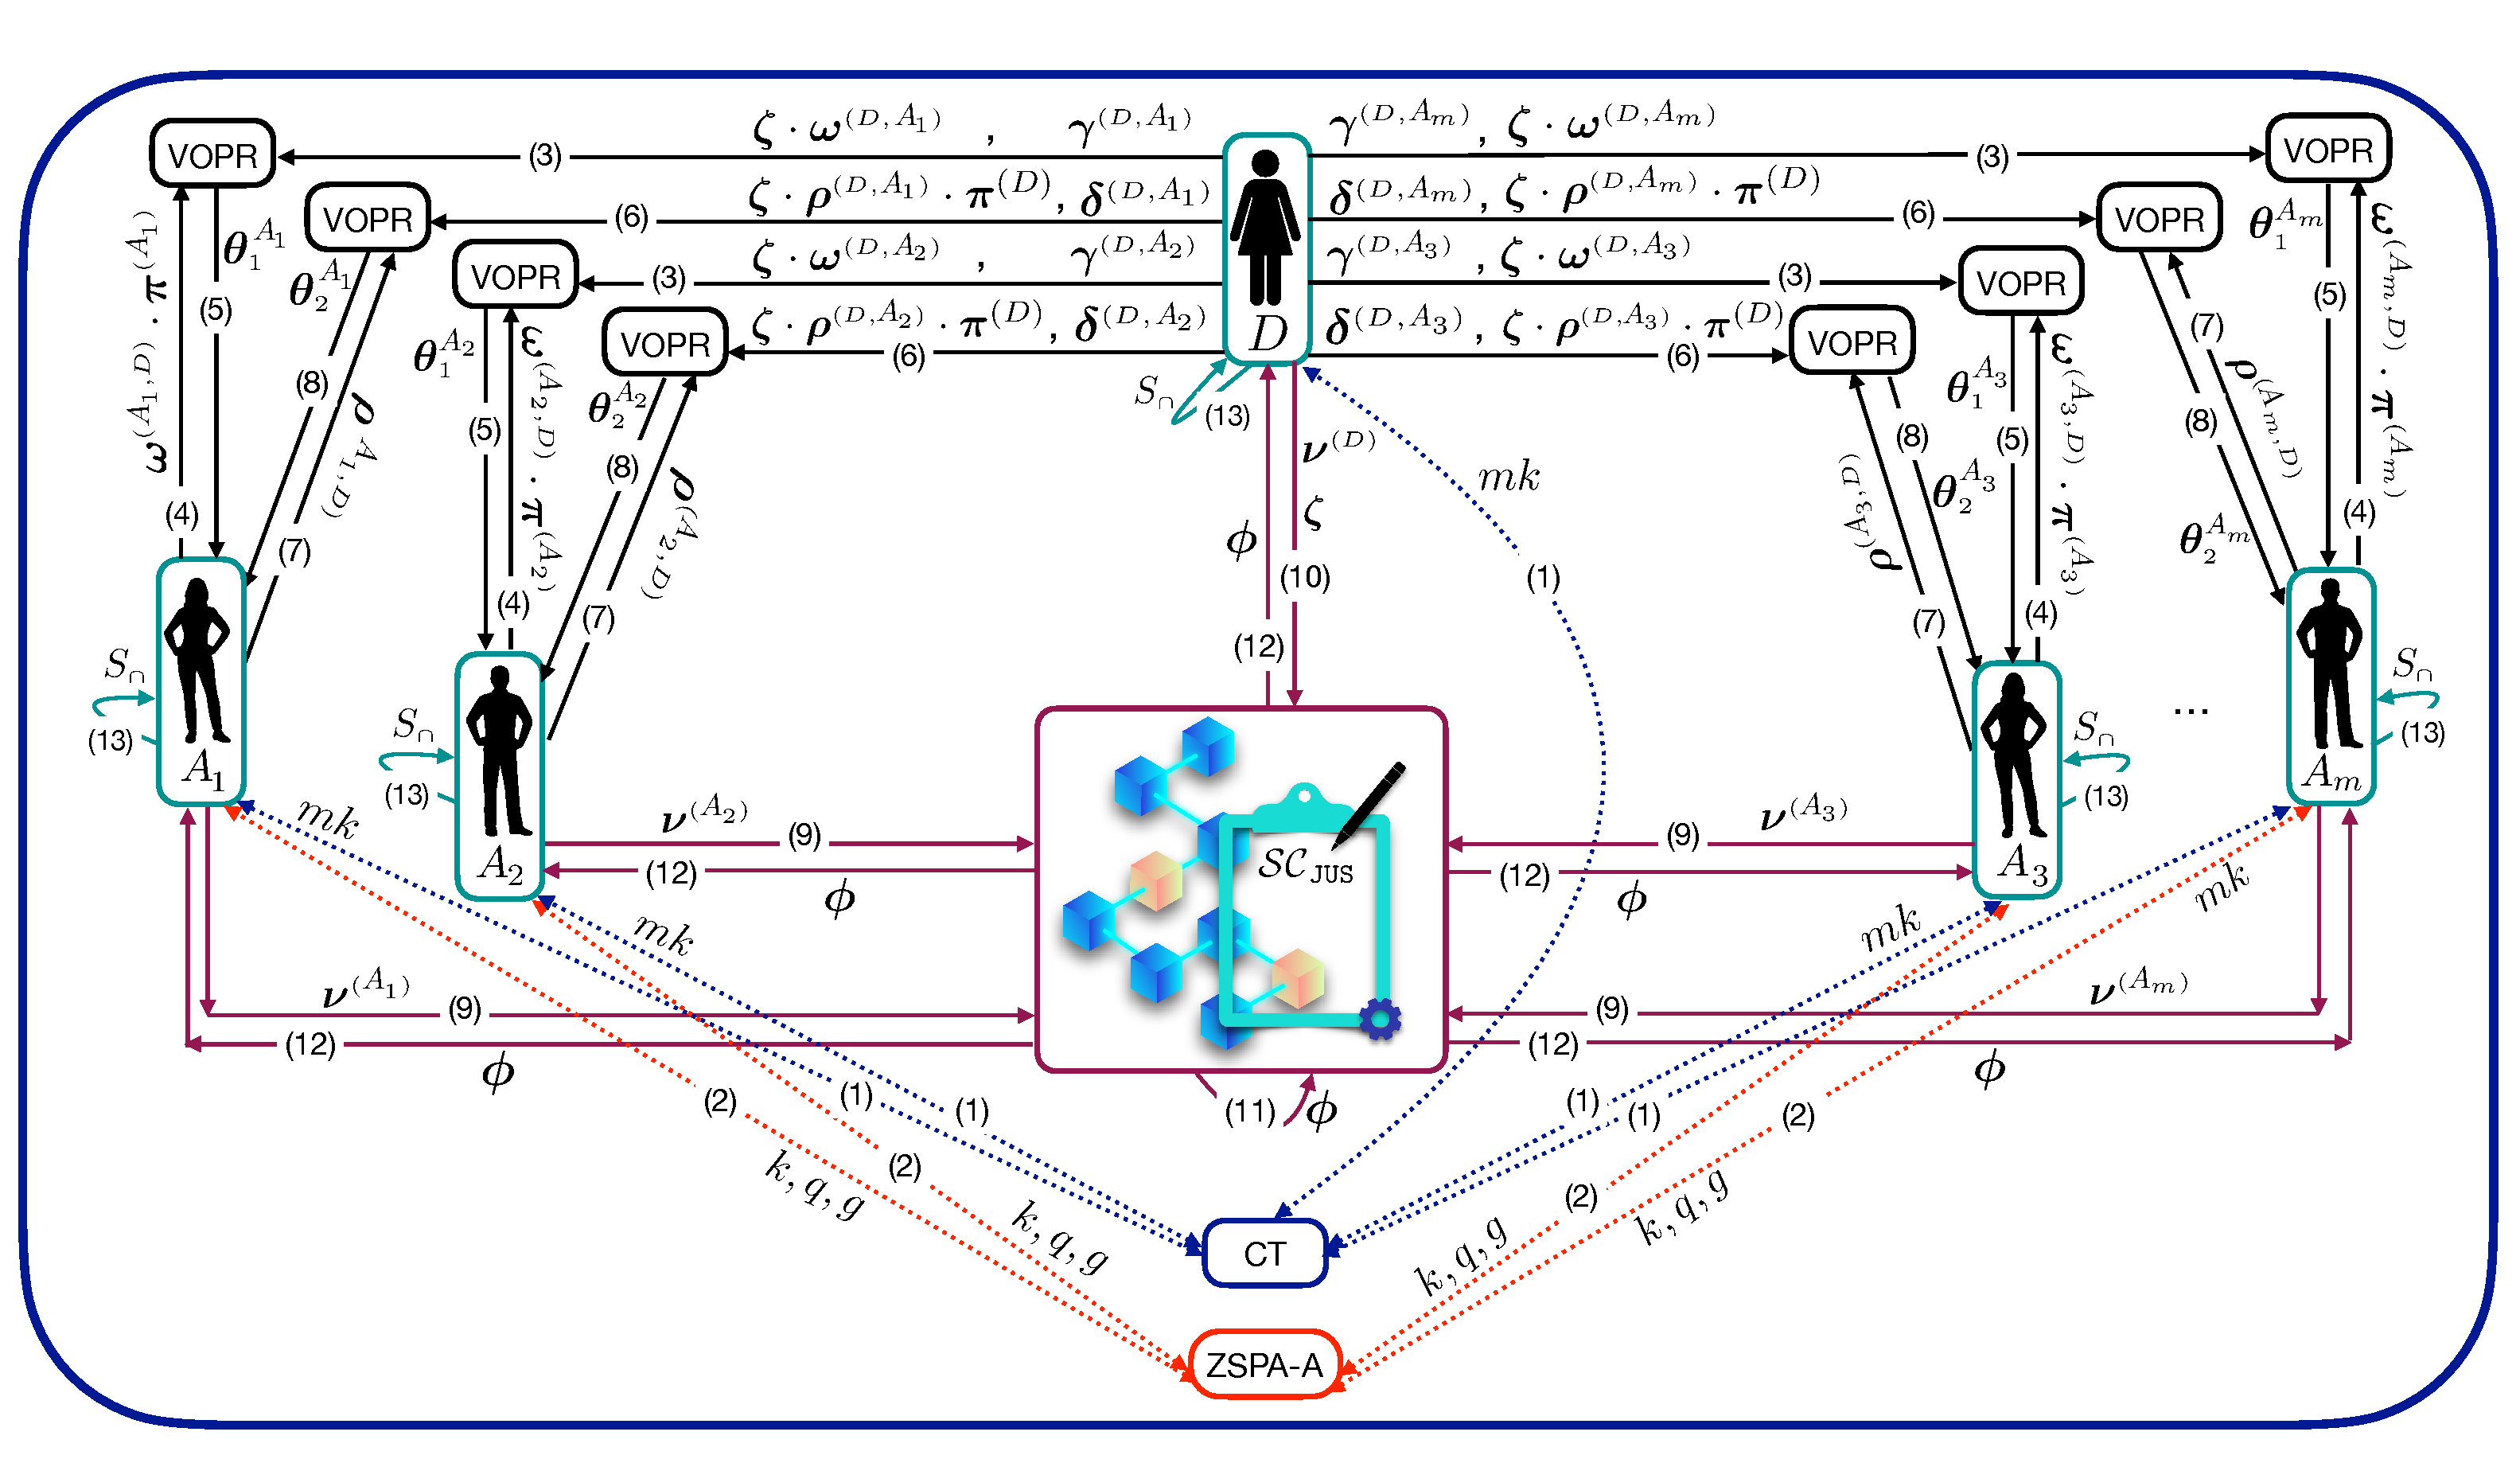
\includegraphics[width=14cm]{Diag-1.pdf}
    \caption{Interaction between parties in \withFai}\label{fig:parties-interactions-in-Jus}
\end{figure}


%%%%%%%%%%%%


One of the novelties of \fpsi is a lightweight verification mechanism which allows a smart contract to efficiently verify the correctness of the clients' messages without being able to learn/reveal the clients' set elements. To achieve this, $D$ randomises each client's polynomials and constructs unforgeable polynomials on the randomised polynomials (in one go). If any client modifies an unforgeable polynomial that it receives and sends the modified polynomial to the smart contract,  then the smart contract would detect it, by checking whether the sum of all clients' (unforgeable) polynomials is divisible by a certain polynomial of degree $1$.  The verification is lightweight because: (i) it does not use any public key cryptography (often computationally expensive), (ii) it needs to perform only polynomial division, and (iii) it can perform batch verification, i.e., it sums all clients randomised polynomials and then checks the result's correctness.


%%%%%%%%%%%%




%
%One of the novelties of F-PS is a lightweight verification mechanism which allows a smart contract to efficiently verify the correctness of the clients' messages without being able to learn/reveal the clients' set elements. To achieve this, the dealer during randomising other clients' polynomials, imposes a MAC-like structure on the randomised polynomials, such that if a client (who receives its randomised polynomial) tampers with it, then the smart contract would detect it. To do the verification, the smart contract needs to only check whether the sum of all clients' randomised polynomials is divisible by a polynomial of degree $1$.  The verification is lightweight because: (i) it does not rely on any public key cryptography (i.e., zero-knowledge proofs), (ii) it needs to perform only polynomial division, and (iii) it can perform batch verification, i.e., instead of individually checking each client's randomised polynomial, it sums all clients randomised polynomials (related to a hash table's bin) and then checks the result's correctness.


% his own
%outsourced dataset and having any knowledge of the other client’s dataset 
%
%
% mainly stems from our observation (stated  in Theorem \ref{proof::unforgeable-poly}) which leads to an  efficient verification mechanism carried out by the contract. 


Now, we describe \fpsi in more detail. First, all clients sign and deploy a  smart contract, \scf. Each of them put a certain amount of deposit into it. Then, they together run \ct to agree on a key, $mk$, that will be used to generate a set of blinding polynomials to hide the final result from the public. Next, each client locally maps its set elements to a hash table and represents the content of each hash table's bin as a polynomial, $\bm\pi$. After that, for each bin, the following steps are taken.  All clients, except $D$, engage in \zspaa to agree on a set of pseudorandom blinding factors such that their sum is zero.  %The clients will use these polynomials to hide from $D$ the polynomials that they will send to \scf. 

Then, $D$ randomises and constructs an unforgeable polynomial on each client's polynomial, $\bm\pi$. To do that, $D$ and every other client engage in \vopr that returns to the client a polynomial. $D$ and every other client invoke \vopr again to randomise $D$'s polynomial. \vopr returns to the client another unforgeable polynomial. Note that the output of \vopr reveals nothing about any client's original polynomial $\bm\pi$, as this polynomial has been blinded/encrypted with another secret random polynomial by $D$, during the execution of \vopr. Each client sums the two polynomials,  blinds the result (using the output of  \zspaa), and sends it to \scf. 



After all of the clients send their input polynomials to \scf, $D$ sends to \scf a \emph{switching polynomial} that will allow \scf to obliviously switch the secret blinding polynomials used by $D$ (during the execution of \vopr) to blind each client's original polynomial $\bm\pi$  to another blinding polynomial that all clients can generate themselves, by using key $mk$.  The switching polynomial is constructed in a way that does not affect the verification of unforgeable polynomials. 




Next, $D$ sends to \scf a secret polynomial, $\bm\zeta$, that will allow \scf to check unforgeable polynomials' correctness. Then, \scf\ sums all clients' polynomials and checks if $\bm\zeta$ can divide the sum. \scf\ accepts the clients' inputs if the polynomial divides the sum; otherwise, it invokes \aud to identify misbehaving parties.  In this case, all honest parties' deposit is refunded to them and the deposit of misbehaving parties is distributed among the honest ones as well. If all clients behave honestly,  then each client can locally find the intersection. To do that, it uses $mk$ to locally remove the blinding polynomial from the sum (that the contract generated), then evaluates the unblinded polynomial at each of its set elements and considers an element in the intersection when the evaluation equals zero. 
%The efficiency of the verification in our protocol  mainly stems from our  observation that if an adversary who know only $xx$ modified the polynomial of the form $xx$ then $\zeta$ will not divide result polynomial after unblinding will not divide with a high probability.  


\subsubsection{Detailed Description of \fpsi.} Below, we elaborate on how \fpsi exactly works (see Table \ref{table:notation-table} for description of the main notations used). 

\begin{enumerate}

%\item[$\bullet$] \textbf{Input:} a pseudorandom function: $\mathtt{PRF}$, a hash table's parameters (i.e., the  total number of bins: $h$ and a bin's capacity: $d$), and clients' sets: $S^{\st (I)}$, where $I\in \bar{P}$.

%\item[$\bullet$] \textbf{Output:}  for every bin of the hash table, it outputs a polynomial: $\phi$, whose roots are  encrypted sets elements (of the bin) in the intersection.
\item\label{gen-FPSI-cont} All clients in $\cl=\{ A_{\st 1},...,   A_{\st m},  D\}$ sign a smart contract: \scf and deploy it to a blockchain. All clients get the deployed contract's address. Also, all clients engage in \ct to agree on a secret master key, $mk$.

\item \label{encode-encrypt} Each client in $\cl$  builds a  hash table,  $\mathtt{HT}$, and inserts the set elements into  it, i.e.,  $\forall i: \mathtt{H}( s_{\st i})={indx}$, then $ s_{\st i}\rightarrow \mathtt{HT}_{\st indx}$. It pads every bin with random dummy elements to $d$ elements (if needed). Then,  for every bin, it constructs a polynomial whose roots are the bin's content: $\bm\pi=\prod\limits^{\st d}_{\st i=1} (x-s'_{\st i})$, where $s'_{\st i}$ is either $s_{\st i}$ or a random value. 
%
\item \label{ZSPA} Every client $ C$ in $\cl\setminus D$, for every bin, agree on $b=3d+3$ vectors of pseudorandom blinding factors: $z_{\st i,j}$, such that the sum of each vector elements is zero, i.e., $\sum\limits^{\st m}_{\st j=1}z_{\st i,j}=0$, where $0\leq i\leq b-1$. To do that, they participate in step \ref{ZSPA::ZSPA-invocation} of \zspaa. By the end of this step, for each bin, they agree on a secret key $k$ (that will be used to generate the zero-sum values) as well as two values stored in $\mathcal{SC}_{\fpsi}$, i.e., $q$: the key's hash value and $g$: a Merkle tree's root. After time $t_{\st 1}$,  $D$ ensures that all other clients have agreed on the vectors (i.e., all provided ``approved''  to the contract). If the check fails, it halts. 
%
\item\label{F-PSI::each-client-deposit} Each client in $\cl$ deposits $\yc+\chc$ amount to $\mathcal{SC}_{\fpsi}$. After time $t_{\st 2}$, every client ensures that in total $(\yc+\chc)\cdot (m+1)$ amount has been deposited. Otherwise, it halts and the clients' deposit is refunded. 







\item  $D$ picks a  random polynomial $\bm\zeta \stackrel{\st\$}\leftarrow \mathbb{F}_{\st p}[X]$ of degree $1$, for each bin.  
It, for each client $C$, allocates to each bin two random polynomials: $\bm\omega^{\st(D,C)}, \bm\rho^{\st (D,C)}\stackrel{\st\$}\leftarrow \mathbb{F}_{\st p}[X]$ of degree $d$, and  two  random polynomials: $\bm\gamma^{\st (D,C)}, \bm\delta^{\st (D,C)} \leftarrow \mathbb{F}_{\st p}[X]$ of degree $3d+1$. Also, each client $C$, for each bin, picks two  random polynomials: $\bm\omega^{\st (C,D)}, \bm\rho^{\st (C,D)}\stackrel{\st\$}\leftarrow \mathbb{F}_{\st p}[X]$ of degree $d$. %It also evaluates each polynomial at every element of $\vv{\bm{x}}$ that results in  $\omega^{  {  {D,C}}}_{\st i}$ and $\rho^{  {  {D,C}}}_{\st i}$.




\item\label{e-psi::D-randomises}  $D$ randomises other clients' polynomials. To do so, for every bin, it invokes an instance of {\vopr} (presented in Fig. \ref{fig:VOPR}) with  each client $  C$; where  $D$ sends $\bm\zeta \cdot \bm\omega^{\st  {  {(D,C)}}}$ and $\bm\gamma^{\st  {  {(D,C)}}}$, while client $ C$ sends $\bm\omega^{\st  {  {(C,D)}}}\cdot \bm\pi^{\st  {  {(C)}}}$ to {\vopr}. Each client $C$, for every bin, receives a blind polynomial of the following form: 

$$\bm\theta^{  {  {(C)}}}_{\st 1}=\bm\zeta \cdot \bm\omega^{\st  {  {(D,C)}}}\cdot \bm\omega^{\st  {  {(C,D)}}}\cdot \bm\pi^{\st  {  {(C)}}}+\bm\gamma^{\st  {  {(D,C)}}}$$
%
 from {\vopr}. If any party aborts, the deposit would be refunded to all parties.

\item\label{e-psi::C-randomises} Each client $    {  C}$ randomises  $ {D}$'s polynomial. To do that, each client $    {  C}$, for each bin,  invokes an instance of {\vopr} with   $ {D}$,    where each client $    {  C}$  sends $\bm\rho^{\st  {  {(C,D)}}}$, while  ${D}$  sends $\bm\zeta\cdot\bm \rho^{\st  {  {(D,C)}}}\cdot \bm\pi^{  {  {(D)}}}$ and $\bm\delta^{\st  {  {(D,C)}}}$ to {\vopr}. Every client   $    {  C}$, for each bin,  receives a blind polynomial of the following form: 

$$\bm\theta^{  {  {(C)}}}_{\st 2}=\bm\zeta \cdot \bm\rho^{\st  {  {(D,C)}}}\cdot \bm\rho^{\st  {  {(C,D)}}}\cdot \bm\pi^{\st  {  {(D)}}}+\bm\delta^{\st  {  {(D,C)}}}$$
 from {\vopr}. If any party aborts, the deposit would be refunded to all parties.


\item\label{blindPoly-C-sends-to-contract} Each client $ C$, for every bin, masks the sum of polynomials $\bm\theta^{\st  {  {(C)}}}_{\st 1}$ and $\bm\theta^{\st  {  {(C)}}}_{\st 2}$  using the blinding factors: $z_{\st i,c}$, generated in step \ref{ZSPA}. Specifically, it computes the following blind polynomial (for every bin):  

$$\bm\nu^{ \st {  {(C)}} }= \bm\theta^{ \st {  {(C)}}}_{\st 1}+\bm\theta^{\st  {  {(C)}}}_{\st 2}+\bm \tau^{\st  {  {(C)}} }$$

where $\bm\tau^{\st  {  {(C)}}}=\sum\limits^{\st 3d+2}_{\st i=0}z_{\st i,c}\cdot x^{\st i}$. Next, it sends  all $\bm\nu^{\st  {  {(C)}} }$ to $\mathcal{SC}_{\fpsi}$. If any party aborts, the deposit would be refunded to all parties.


%\item Client $    {  D}$ ensures all clients have sent their inputs to $\mathcal{SC}_{  {   {F-PSI}}}$. In the case where $m'$ parties do not provide their inputs, client $    {  D}$ aborts. In this case, the rest (including the dealer) get their deposit back. Also,  the deposit of the parties who did not send  inputs would be evenly distributed among the rest. The total amount each party above receives is: $y+\frac{m'\cdot y}{m-m'}$




%%
%\item Client $    {  D}$ and each client $    {  C}$ collaboratively, for each bin, generate a polynomial that will be used to (obliviously) check if  $    {  C}$ misbehaved during the computation of each $\bm\nu^{  {  {(C)}} }$. To do so, for every bin, client $    {  D}$ invokes an instance of $\mathtt{VOPR}$ with  each client $    {  C}$, where  client $    {  D}$ sends: $\bm\zeta$, while client $    {  C}$ sends $\bm\xi^{  {  {(C)}}}$ and $-\bm\tau^{  {  {(C)}}}$   to $\mathtt{VOPR}$, where $\bm\xi^{  {  {(C)}}}$ is a random polynomial of degree $3d+1$. Client $    {  D}$ for each  $    {  C}$'s bin recives the following polynomial: 
%%
%$$\bm\mu^{  {  {(D,C)}}} = \bm\zeta\cdot \bm\xi^{  {  {(C)}}}-\bm\tau^{  {  {(C)}}}$$
%%




\item\label{f-psi::D-gen-random-poly} ${D}$ ensures all clients sent their inputs to $\mathcal{SC}_{\fpsi}$. If the check fails, it halts and the deposit would be refunded to all parties. It allocates a fresh pseudorandom polynomial $\bm\gamma'$ of degree $3d$, to each bin. To do so, it uses $mk$ to derive a key for each bin: $k_{\st  { {indx}}}=\mathtt{PRF}(mk, {    {   {indx}}})$ and then uses the derived key to generate $3d+1$ pseudorandom coefficients $g_{\st  { {j,indx}}}=\mathtt{PRF}(k_{\st  { {indx}}}, j)$ where $ 0\leq j \leq 3d$. Also, for each bin, it allocates a fresh random polynomial:  $\bm\omega'^{\st  {  {(D)}}}$ of degree $d$. 

\item\label{f-psi::D-gen-switching-poly}  $ {D}$,  for every bin, computes a polynomial of the form:  

$$\bm\nu^{\st  {  {(D)}}}=\bm\zeta \cdot  \bm\omega'^{\st  {  {(D)}}}\cdot \bm\pi^{\st  {  {(D)}} }-\sum\limits^{\st  {   A}_{\st  {   m}}}_{\st   {  {C }= }   {   A}_{\st  {  1}}}(\bm\gamma^{\st  {  {(D,C)}}} + \bm\delta^{\st  {  {(D,C)}}}) + \bm\zeta \cdot \bm\gamma'$$ 
It sends to $\mathcal{SC}_{\fpsi}$  polynomials $\bm\nu^{\st  {  {(D)}}}$ and $\bm\zeta$, for each bin.

 \item\label{compute-res-poly}  $\mathcal{SC}_{\fpsi}$ takes the following steps:
 \begin{enumerate}
 \item for every bin, sums all related polynomials  provided by all clients in $\bar{P}$:
 
 \begin{equation*}
\begin{split}
 \bm\phi&= \bm\nu^{\st  {  {(D)}} }+\sum\limits^{\st  {   A}_{\st  {   m}}}_{\st   {  {C }= }   {   A}_{\st  {  1}}}\bm\nu^{\st  {  {(C)}} }\\
 &= \bm\zeta\cdot \bigg(\bm\omega'^{\st  {  {(D)}}}\cdot \bm\pi^{\st  {  {(D)}} } +\sum\limits^{\st  {   A}_{  {   m}}}_{\st  {  {C }= }   {   A}_{\st  {  1}}}(\bm\omega^{\st  {  {(D,C)}}} \cdot \bm\omega^{\st  {  {(C,D)}}}\cdot \bm\pi^{\st  {  (C)}}) +\bm\pi^{\st  {  {(D)}}}\cdot\sum\limits^{\st  {   A}_{ \st {   m}}}_{\st  {C= }   {   A}_{\st  {  1}}}(\bm\rho^{\st  {  {(D,C)}}} \cdot \bm\rho^{\st  {  {(C,D)}}}) + \bm\gamma'\bigg)
  \end{split}
\end{equation*}
% \item\label{F-PSI:detect-misbehaving-party} ensures that, for every bin, $\bm\zeta$ divides $\bm\phi$. Otherwise, it aborts and Arbiter protocol (presented in Fig. \ref{fig:arbiter}) is invoked to find misbehaving parties.
 
  \item\label{F-PSI:detect-misbehaving-party} checks whether, for every bin, $\bm\zeta$ divides $\bm\phi$. If the check passes, it sets $Flag=True$. Otherwise, it sets $Flag=False$. 
  
   %aborts and Arbiter protocol (presented in Fig. \ref{fig:arbiter}) is invoked to find misbehaving parties.
 
 
% \item if the check passes (i.e., $Flag=True$), each party gets back its deposit (i.e., $y$ amount).
 \end{enumerate}
 
\item\label{F-PSI::flag-is-true} If the above check passes (i.e., $Flag=True$), then the following steps are taken:

\begin{enumerate}
 \item $\mathcal{SC}_{\fpsi}$ sends back each party's deposit, i.e., $\yc+\chc$ amount.
 
  \item each client (given $\bm\zeta$ and $mk$) finds the elements in the intersection as follows. 
  \begin{enumerate}
  \item derives a bin's pseudorandom polynomial, $\bm\gamma'$, from $mk$. 
  
  \item removes the blinding polynomial from each bin's polynomial: 
  
  $$\bm\phi'=\bm\phi-\bm\zeta\cdot \bm\gamma'$$ 
  
  \item\label{F-PSI::find-intersection} evaluates each bin's unblinded polynomial at every element $s_{\st i}$ belonging to that bin and considers the element in the intersection if the evaluation is zero: i.e., $\bm\phi'(s_{\st i})=0$.
 
 \end{enumerate}
 
 
 \end{enumerate}
 
 \item\label{F-PSI::flag-is-false} If the check does not pass (i.e., $Flag=False$), then the following steps are taken.
 
 

 
 \begin{enumerate}
 

 \item\label{auditor}  \aud asks every client $    {  C}$ to send to it the  $\mathtt{PRF}$'s key (generated in step \ref{ZSPA}), for every bin. It inserts the keys to $\vv k$.  It generates a list $\bar L$ initially empty. Then, for every bin,  \aud takes step \ref{ZSPA-A::Auditor-computation} of \zspaa, i.e., invokes  $\mathtt{Audit}( \vv{{k}},  q, \bm\zeta, 3d+3, g)\rightarrow (L, \vv{{\mu}})$.  Every time it invokes $\mathtt{Audit}$, it appends the elements of returned $L$ to $\bar L$.  \aud for each bin sends  $ \vv{{\mu}}$ to $\mathcal{SC}_{\fpsi}$. It also sends  to $\mathcal{SC}_{\fpsi}$ the list $\bar L$ of all misbehaving clients detected so far.
 

 
 \item to  help identify further  misbehaving clients, $D$ takes the following steps,  for each bin of client $    {  C}$ whose ID is not in $\bar L$.   
 \begin{enumerate}
 \item\label{gen-unmaking-poly} computes polynomial $\bm\chi^{  {  {(D, C)}}}$ as follows. 
 
 $$\bm\chi^{ \st {  {(D, C)}}}=\bm\zeta\cdot \bm\eta^{ \st {  {(D,C)}}}-(\bm\gamma^{ \st {  {(D,C)}}}+\bm\delta^{ \st {  {(D,C)}}})$$
 
 %+\bm\mu^{  {  {(D, C)}}}
 
  where $\bm\eta^{ \st {  {(D,C)}}}$ is a fresh random polynomial of degree $3d+1$. 
  
  \item\label{send-unmaking-poly} sends  polynomial $\bm\chi^{ \st {  {(D, C)}}}$ to  $\mathcal{SC}_{\fpsi}$. 
  

 \end{enumerate}
  Note, if $\bar L$ contains all clients' IDs, then $D$ does not need to take the above steps \ref{gen-unmaking-poly} and \ref{send-unmaking-poly}. 
 %%%%%%%%%%%%%%%%%%%%%%
 
 \item  $\mathcal{SC}_{\fpsi}$,   takes the following steps to check if the client misbehaved,  for each bin of client $    {  C}$ whose ID is not in $\bar L$.
 
 %for each client $    {  C}$'s bin, takes the following steps to check if the client misbehaved.
 
  \begin{enumerate}
  
 \item computes  polynomial $\bm\iota^{\st  {  {(C)}}}$ as follows: 
 
  \begin{equation*}
\begin{split}
 \bm\iota^{ \st {  {(C)}}}&=\bm\chi^{\st  {  {(D, C)}}}+\bm\nu^{\st  {  {(C)}}} +\bm\mu^{ \st {  {(C)}}} \\ 
 &=\bm\zeta\cdot(\bm\eta^{ \st {  {(D,C)}}} + \bm\omega^{ \st {  {(D,C)}}}\cdot \bm\omega^{ \st {  {(C,D)}}}\cdot \bm\pi^{ \st {  {(C)}}}+\bm\rho^{ \st {  {(D,C)}}}\cdot \bm\rho^{ \st {  {(C,D)}}}\cdot \bm\pi^{ \st {  {(D)}}}+\bm\xi^{ \st {  {(C)}}})
 \end{split}
\end{equation*}

 where $\bm\mu^{ \st {  {(C)}}} \in \vv{\mu}$ generated and sent to $\mathcal{SC}_{\fpsi}$  by \aud in step \ref{auditor}.   
  \item checks if $\bm\zeta$  divides $\bm\iota^{ \st {  {(C)}}}$. If the check fails, it appends the client's ID to  a list $ L'$.
  %
  \end{enumerate}
   If $\bar L$ contains all clients' IDs, then $\mathcal{SC}_{\fpsi}$ does not take the above two steps. 

 %
   \item  $\mathcal{SC}_{\fpsi}$  refunds the honest parties' deposit. Also, it retrieves the total amount of  $\chc$ from the deposit of dishonest clients (i.e., those clients whose IDs are in $\bar L$ or $L'$) and sends it to \aud.  It also splits the remaining deposit of the misbehaving parties among the honest ones. Thus, each honest client  receives $\yc+\chc+\frac{m'\cdot (\yc+\chc)-\chc}{m-m'}$ amount in total, where $m'$ is the total number of misbehaving parties.
 
 
%  \item  $\mathcal{SC}_{  {   {F-PSI}}}$  refunds the honest parties' deposit and splits the deposit of the misbehaving parties (i.e., those clients whose IDs are in $\bar L$ or $L'$)  among the honest ones. Thus, each honest party would receive $y+\frac{m'\cdot y}{m-m'}$ amount in total, where $m'$ is the total number of misbehaving parties.
 %%%%%%%%%%%%%%%%%%%%%
  \end{enumerate}
  
% \item If  $Flag=False$,  then $\mathcal{SC}_{  {   {F-PSI}}}$,  for each client $    {  C}$'s bin, takes the following steps:
% 
%  \begin{enumerate}
%  
% \item computes the following polynomial: 
% 
%  \begin{equation*}
%\begin{split}
% \bm\iota^{  {  {(C)}}}&=\bm\chi^{  {  {(D, C)}}}+\bm\nu^{  {  {(C)}}} \\ 
% &=\bm\zeta\cdot(\bm\eta^{  {  {(D,C)}}} + \bm\omega^{  {  {(D,C)}}}\cdot \bm\omega^{  {  {(C,D)}}}\cdot \bm\pi^{  {  {(C)}}}+\bm\rho^{  {  {(D,C)}}}\cdot \bm\rho^{  {  {(C,D)}}}\cdot \bm\pi^{  {  {(D)}}}+\bm\xi^{  {  {(C)}}})
% \end{split}
%\end{equation*}
% 
%  \item checks if $\bm\zeta$  divides $\bm\iota^{  {  {(C)}}}$. If does not, it appends the client's ID to a  list, $L$.
%  
%  \end{enumerate}
 
% \begin{equation*}
%\begin{split}
% \bm\iota^{  {  {(C)}}}&=\bm\zeta\cdot \bm\eta^{  {  {(D,C)}}}-(\bm\gamma^{  {  {(D,C)}}}+\bm\delta^{  {  {(D,C)}}})+\bm\nu^{  {  {(C)}}}-\sum\limits^{\st 3d+1}_{\st i=0}z_{\st i,c}\cdot x^{\st i} \\ &=\bm\zeta\cdot(\bm\eta^{  {  {(D,C)}}} + \bm\omega^{  {  {(D,C)}}}\cdot \bm\omega^{  {  {(C,D)}}}\cdot \bm\pi^{  {  {(C)}}}+\bm\rho^{  {  {(D,C)}}}\cdot \bm\rho^{  {  {(C,D)}}}\cdot \bm\pi^{  {  {(D)}}})
% \end{split}
%\end{equation*}
%  \item checks if $\bm\zeta$ can divide $\bm\iota^{  {  {(C)}}}$. If can not, it appends the client's ID to $L$.
% 
 

 
 
 
% \item Each client (given $\bm\zeta$ and $k_{\st 1}$), finds the elements in the intersection as follows. First, it derives a bin's pseudorandom polynomial: $\bm\gamma'$ from $k_{\st 1}$.  Next, it removes the blinding polynomial from each bin's polynomial: $\bm\phi'=\bm\phi-\bm\zeta\cdot \bm\gamma'$. Then, it evaluates each bin's unblinded polynomial at every  element belonging to that bin and considers the element in the intersection if the evaluation is zero: i.e. $\bm\phi'(s^{  {  {(I)}}}_{\st i})=0$
 
  \end{enumerate}
 
% the result: $cccc$ by locally evaluating the result polynomial: $\phi(x)$, at every  encrypted element, $e^{  {  {(I)}}}_{\st i}$, it has and considering the elements in the intersection if the following equation holds.  $\forall i, 1\leq i\leq d: \phi(e^{  {  {(I)}} }_{\st i})-\zeta(e^{  {  {(I)}}}_{\st i})\cdot \gamma'(e^{  {  {(I)}}}_{\st i})=0$.
 
 
 
%\begin{remark} After the Arbiter detects  misbehaving parties,  in step \ref{F-PSI:detect-misbehaving-party},  it sends their ID's to $\mathcal{SC}_{  {   {F-PSI}}}$ which refunds the honest parties' deposit and splits the misbehaving parties' deposit among the honest ones. Thus, each honest party would receive: $y+\frac{m'\cdot y}{m-m'}$ amount in total, where $m'$ is the total number of misbehaving parties.
% \end{remark}
 
 

%\begin{remark}
One may be tempted to replace $\withFai$ with a scheme in which all clients send their encrypted sets to a server (potentially semi-honest and plays \aud's role) which computes the result in a privacy-preserving manner.  We highlight that the main difference is that in this (hypothetical) scheme the server is \emph{always involved};  whereas, in our protocol, \aud remains offline as long as the clients behave honestly and it is invoked only when the contract detects misbehaviours.  
%\end{remark}
 
 
 Next, we present a theorem that formally states the security of \fpsi. 
 
 \begin{theorem}\label{theorem::F-PSI-security}
Let polynomials $\bm\zeta$, $\bm\omega$, and $\bm\gamma$ be three secret uniformly random polynomials. If  $\bm\theta=\bm\zeta\cdot \bm\omega\cdot\bm \pi+\bm \gamma \bmod p$ is an unforgeable polynomial (w.r.t. Theorem \ref{proof::unforgeable-poly}), \zspaa, \vopr,  $\mathtt{PRF}$, and smart contracts are secure, then \fpsi securely realises  $f^{\st \text{PSI}}$ with $Q$-fairness (w.r.t. Definition \ref{def::PSI-Q-fair}) in the presence of $m-1$  active-adversary clients (i.e., $A_{\st j}$s) or a passive dealer client, passive auditor, or passive public. 
 \end{theorem}
 






 % !TEX root =main.tex


\section{Proof of \fpsi}\label{sec::F-PSI-proof}



In this section, we prove Theorem \ref{theorem::F-PSI-security}, i.e., the security of \fpsi. 


\begin{proof}
%
We prove Theorem  \ref{theorem::F-PSI-security} by considering the case where each party is corrupt, at a time.

\noindent\textbf{Case 1: Corrupt $m-1$ clients in $\{  {  A}_{ \st {   1}}, ...,   {  A}_{ \st {   m}}\}$}.  Let $P'$ be a set of at most $m-1$ corrupt clients, where $P'\subset \{  {  A}_{ \st {   1}}, ...,   {  A}_{ \st {   m}}\}$. Let set $\hat P$ be defined as follows: $\hat P=\{  {  A}_{ \st {   1}}, ...,   {  A}_{ \st {   m}}\}\setminus P'$. Also, let $\mathsf{Sim}^{\st\fpsi}_{\st A}$ be the simulator, which uses a subroutine adversary, $\mathcal{A}$.  Below, we explain how $\mathsf{Sim}^{\st \fpsi}_{\st A}$ (which receives the input sets of honest dealer $D$ and honest client(s) in $\hat P$) works. 


\begin{enumerate}
%
\item constructs and deploys a smart contract. It sends the contract's address to $\mathcal{A}$. 
%
\item simulates \ct and receives the output value, $ {mk}$, from its functionality, $f_{\st \ct}$.
%
\item\label{sim::ZSPA-A-invocation} simulates \zspaa for each bin and receives the output value, $( k,  g,  q)$, from its functionality, $f^{\st \zspaa}$.
%
\item deposits in the contract the total amount of $(\yc+\chc)\cdot (m-|P'|+1)$ coins on behalf of $D$ and honest client(s) in $\hat P$. It sends to $\mathcal{A}$ the amount deposited in the contract. 
%
\item checks if $\mathcal{A}$ has deposited $(\yc+\chc)\cdot |P'|$ amount. If the check fails, it instructs the ledger to refund the coins that every party deposited and sends message $abort_{\st 1}$ to TTP (and accordingly to all parties); it outputs whatever $\mathcal{A}$ outputs and then halts. 

%
\item picks a random polynomial ${\bm\zeta}$ of degree $1$, for each bin. Also, $\mathsf{Sim}^{\st \fpsi}_{\st A}$, for each client $  {  C}\in \{  {  A}_{ \st {   1}}, ...,   {  A}_{ \st {   m}}\}$ allocates to each bin two random polynomials: (${\bm\omega}^{ \st {  {(D,C)}}}, {\bm\rho}^{ \st {  {(D,C)}}}$) of degree $d$ and   two random polynomials: (${\bm\gamma}^{ \st {  {(D,C)}}}$, ${\bm\delta}^{ \st {  {(D,C)}}}$) of degree $3d+1$. Moreover, $\mathsf{Sim}^{\st \fpsi}_{\st A}$ for every honest client $C'\in \hat P$, for each bin, picks two random polynomials: (${\bm\omega}^{ \st {  {(C',D)}}}$, ${\bm\rho}^{ \st {  {(C',D)}}}$) of degree $d$. %Note, all polynomials are picked from $\mathbb{F}_{\st p}[X]$. 
%
\item\label{F-PSI::sim-A-first-VOPR-invocation} simulates \vopr using inputs ${\bm\zeta} \cdot {\bm\omega}^{ \st {  {(D,C)}}}$ and ${\bm\gamma}^{ \st {  {(D,C)}}}$ for each bin. Accordingly, it receives the inputs of clients $C''\in P'$, i.e., ${\bm\omega}^{ \st {  {(C'',D)}}}\cdot {\bm\pi}^{ \st {  {(C'')}}}$, from its functionality $f^{\st \vopr}$, for each bin.  
%
%\item receives from $\mathcal{A}$ the outputs of VOPR for every client $C'' \in P'$. It ensures the output for every $C''$ has been provided. Otherwise, it halts.  
%
\item extracts the roots of polynomial ${\bm\omega}^{ \st {  {(C'',D)}}}\cdot {\bm\pi}^{ \st {  {(C'')}}}$ for each bin and appends those roots that are in the sets universe to a new set $S^{\st(C'')}$. 
%
\item simulates  \vopr again using inputs ${\bm\zeta}\cdot {\bm \rho}^{ \st {  {(D,C)}}}\cdot {\bm\pi}^{ \st {  {(D)}}}$ and ${\bm\delta}^{ \st {  {(D,C)}}}$, for each bin. %It receives the inputs of clients $C''\in P'$, i.e., $ {\bm\rho}^{ \st {  {(C'',D)}}}$, from $f^{\st \text{VOPR}}$, for each bin. 
%
\item sends to TTP the input sets of all parties; namely, (i) client $D$'s input set: $S^{\st (D)}$, (ii) honest clients' input sets: $S^{\st (C')}$ for all $C'$ in $\hat P$, and (iii) $\mathcal{A}$'s input sets: $S^{\st(C'')}$, for all $C''$ in $P'$.  For each bin, it receives the intersection set, $S_{\st\cap}$, from TTP. 
%
\item represents the intersection set for each bin as a polynomial, ${\bm \pi}$, as follows: ${\bm \pi}=\prod\limits^{\st |S_{\st\cap}|}_{\st i=1 }(x-s_{\st i})$, where $s_{\st i}\in S_{\st\cap}$. 

%
\item constructs polynomials ${\bm\theta}^{ \st {  {(C')}}}_{\st 1}={\bm\zeta} \cdot {\bm\omega}^{ \st {  {(D,C')}}}\cdot {\bm\omega}^{ \st {  {(C',D)}}}\cdot {\bm\pi}+{\bm\gamma}^{ \st {  {(D,C')}}}, {\bm\theta}^{ \st {  {(C')}}}_{\st 2}=  {\bm\zeta} \cdot  {\bm\rho}^{ \st {  {(D,C')}}}\cdot  {\bm\rho}^{ \st {  {(C',D)}}}\cdot  {\bm\pi}+  {\bm\delta}^{ \st {  {(D,C')}}}$, and $ {\bm\nu}^{ \st {  {(C')}} }=  {\bm\theta}^{ \st {  {(C')}}}_{\st 1}+ {\bm\theta}^{ \st {  {(C')}}}_{\st 2}+ {\bm \tau}^{ \st {  {(C')}} }$, for each bin and each honest client $C'\in\hat P$, where $ {\bm\tau}^{ \st {  {(C)}}}=\sum\limits^{\st 3d+2}_{\st i=0}z_{\st i,c}\cdot x^{\st i}$ and each $z_{\st i,c}$ is derived from $  k$. 
%
\item sends to $\mathcal{A}$ polynomial  $ {\bm\nu}^{ \st {  {(C')}} }$ for each bin and each client $C'$. 
%
\item\label{F-PSI::sim-A-receive-nu-from-adv} receives $ {\bm\nu}^{ \st {  {(C'')}} }$  from $\mathcal{A}$, for each bin and each client $C''\in P'$. It ensures that the output for every $C''$ has been provided. Otherwise, it halts. 
%
\item if there is any abort within steps \ref{F-PSI::sim-A-first-VOPR-invocation}--\ref{F-PSI::sim-A-receive-nu-from-adv}, then it sends $abort_{\st 2}$ to TTP and instructs the ledger to refund the coins that every party deposited.  It outputs whatever $\mathcal{A}$ outputs and then halts. 
%
\item constructs polynomial  $ {\bm\nu}^{ \st {  {(D)}}}= {\bm\zeta} \cdot   {\bm\omega'}^{ \st {  {(D)}}}\cdot  {\bm\pi} - \sum\limits^{ \st {   A}_{ \st {   m}}}_{  \st {  {C }= }  \st {   A}_{ \st {  1}}}( {\bm\gamma}^{ \st {  {(D,C)}}} +  {\bm\delta}^{ \st {  {(D,C)}}}) +  {\bm\zeta} \cdot  {\bm\gamma'}$ for each bin, where $ {\bm\omega'}^{ \st {  {(D)}}}$ is a fresh random polynomial of degree $d$ and $ {\bm\gamma'}$ is a pseudorandom polynomial derived from $  {mk}$.
%
\item sends to $\mathcal{A}$ polynomials $ {\bm\nu}^{ \st {  {(D)}}}$ and $ {\bm\zeta}$ for each bin. 
%
\item given each $ {\bm\nu}^{ \st {  {(C'')}} }$, computes polynomial $ {\bm\phi'}$ as follows $ {\bm\phi'} = \sum\limits_{\st \forall C''\in P'} {\bm\nu}^{ \st {  {(C'')}} }- \sum\limits_{\st \forall C''\in P'}( {\bm\gamma}^{ \st {  {(D,C'')}}} +  {\bm\delta}^{ \st {  {(D,C'')}}})$, for every bin. Then, $\mathsf{Sim}^{\st \fpsi}_{\st A}$ checks whether  $ {\bm\zeta}$  divides ${\bm\phi'}$, for every bin. If the check passes, it sets $Flag=True$. Otherwise, it sets $Flag=False$. 
%
\item if $Flag=True$:

\begin{enumerate}
%
 \item instructs the ledger to send back each party's deposit, i.e., $\yc+\chc$ amount. It sends a message $deliver$ to TTP.  
 %
 \item outputs whatever $\mathcal{A}$ outputs and then halts. 
 %
 \end{enumerate}
%
\item if $Flag=False$: 
%
\begin{enumerate}
%
 \item receives $|P'|$ keys of the $\mathtt{PRF}$ from $\mathcal{A}$, i.e., $\vv k'=[   k'_{\st 1}, ...,   k'_{\st |P'|}]$, for every bin. %, which should be the output of $f^{\st \text{ZSPA-A}}$ in step \ref{sim::ZSPA-A-invocation} above. 
%
\item checks whether the following equation holds: $  k'_{\st j}=  k$, for every $  k'_{\st j}\in\vv k'$. Note that $  k$ is the output of $f^{\st \zspaa}$ generated in step \ref{sim::ZSPA-A-invocation}. It constructs an empty list $  L'$ and appends to it the indices (e.g., $j$) of the keys that do not pass the above check. 
%
\item simulates \zspaa and receives from $f^{\st \zspaa}$ the output that contains a vector of random polynomials, $\vv{\mu}'$, for each valid key. 
%
\item sends to  $\mathcal{A}$, the list $  L'$ and vector  $\vv{\mu}'$, for every bin. 
%
\item  for each bin of client $  {  C}$ whose index (or ID) is not in $  L'$ computes polynomial $ {\bm\chi}^{ \st {  {(D, C)}}}$ as follows: 
 %
 $ {\bm\chi}^{ \st {  {(D, C)}}}= {\bm\zeta}\cdot  {\bm\eta}^{ \st {  {(D,C)}}}-( {\bm\gamma}^{ \st {  {(D,C)}}}+ {\bm\delta}^{ \st {  {(D,C)}}})$,   where $ {\bm\eta}^{ \st {  {(D,C)}}}$ is a fresh random polynomial of degree $3d+1$. Note, $C$ includes both honest and corrupt clients, except those clients whose index is in  $  L'$. $\mathsf{Sim}^{\st \fpsi}_{\st A}$ sends every polynomial $ {\bm\chi}^{ \st {  {(D, C)}}}$ to  $\mathcal{A}$. 
 %
 \item given each $ {\bm\nu}^{ \st {  {(C'')}} }$ (by $\mathcal{A}$ in step \ref{F-PSI::sim-A-receive-nu-from-adv}), computes polynomial $ {\bm\phi'}^{ \st {  {(C'')}} }$ as follows: ${\bm\phi'}^{ \st {  {(C'')}} } =  {\bm\nu}^{ \st {  {(C'')}} }-  {\bm\gamma}^{ \st {  {(D,C'')}}} -  {\bm\delta}^{ \st {  {(D,C'')}}}$, for every bin. Then, $\mathsf{Sim}^{\st \fpsi}_{\st A}$ checks whether  $ {\bm\zeta}$  divides $ {\bm\phi'}^{ \st {  {(C'')}} }$, for every bin. It appends the index of those clients that did not pass the above check to a new list, $  L''$. Note that $  L'\cap   L''=\bot$.
%
\item if  $  L'$ or $  L''$ is not empty, then it instructs the ledger: (i) to refund the coins of those parties whose index is not in $  L'$ and $  L''$, (ii) to retrieve $\chc$ amount from the adversary (i.e., one of the parties whose index is in one of the lists) and send the $\chc$ amount to the auditor, and (iii) to compensate each honest party (whose index is not in the two lists)  $\frac{m'\cdot (\yc+\chc)-\chc}{m-m'}$ amount, where $m'=|  L'|+|  L''|$.  Then, it sends  message $abort_{\st 3}$ to TTP. 
%
\item outputs whatever $\mathcal{A}$ outputs and halts. 
 %
 \end{enumerate}
%
\end{enumerate}

Next, we show that the real and ideal models are computationally indistinguishable. We first focus on the adversary’s output. In the real and ideal models, the adversary sees the transcripts of ideal calls to $f_{\st \ct}$ as well as this functionality outputs, i.e., $mk$. Due to the security of \ct (as we are in the $f_{\st \ct}$-hybrid world), the transcripts of $f_{\st \ct}$ in both models have identical distribution, so have the random output of $f_{\st \ct}$, i.e., $mk$. The same holds for (the transcripts and) outputs (i.e., $(  k,   g,   q)$) of $f^{\st \zspaa}$ that the adversary observes in the two models. Also, the deposit amount is identical in both models. Thus, in the case where $abort_{\st 1}$ is disseminated at this point; the adversary's output distribution in both models is identical. 



The adversary also observes (the transcripts and) outputs of ideal calls to $f^{\st \vopr}$ in both models, i.e., output ($\bm\theta^{ \st {  {(C'')}}}_{\st 1}=\bm\zeta \cdot \bm\omega^{ \st {  {(D, C'')}}}\cdot \bm\omega^{ \st {  {(C'', D)}}}\cdot \bm\pi^{ \st {  {(C'')}}}+\bm\gamma^{ \st {  {(D,C'')}}}, \bm\theta^{ \st {  {(C'')}}}_{\st 2}=\bm\zeta \cdot \bm\rho^{ \st {  {(D, C'')}}}\cdot \bm\rho^{ \st {  {(C'',D)}}}\cdot \bm\pi^{ \st {  {(D)}}}+\bm\delta^{ \st {  {(D, C'')}}}$) for each corrupted client $C''$. However, due to the security of \vopr, the $\mathcal{A}$'s view, regarding \vopr, in both models have identical distribution.  
%
In the real model, the adversary observes the polynomial ${\bm\nu}^{ \st {  {(C)}}}$ that each honest client $C$ stores in the smart contract. Nevertheless, this is a blinded polynomial comprising of two uniformly random blinding polynomials (i.e., $\bm\gamma^{ \st {  {(D,C)}}}$ and $\bm\delta^{ \st {  {(D,C)}}}$) unknown to the adversary. In the ideal model, $\mathcal{A}$ is given polynomial  $ {\bm\nu}^{ \st {  {(C')}}}$ for each honest client $C'$. This polynomial has also been blinded via two uniformly random polynomials (i.e., $ {\bm\gamma}^{ \st {  {(D, C')}}}$ and $ {\bm\delta}^{ \st {  {(D, C')}}}$) unknown to $\mathcal{A}$. Thus, ${\bm\nu}^{ \st {  {(C)}}}$ in the real model and $ {\bm\nu}^{ \st {  {(C)}}}$ in the ideal model have identical distributions. As a result, in the case where $abort_{\st 2}$ is disseminated at this point; the adversary's output distribution in both models is identical. 



Furthermore, in the real world, the adversary observes polynomials ${\bm\zeta}$ and  $\bm\nu^{ \st {  {(D)}}}$  that  $D$ stores in the smart contract. Nevertheless, ${\bm\zeta}$ is a uniformly random polynomial, also polynomial $\bm\nu^{ \st {  {(D)}}}$ has been blinded; its blinding factors are the additive inverse of  the sum of the random polynomials $\bm\gamma^{ \st {  {(D,C)}}}$ and $\bm\delta^{ \st {  {(D,C)}}}$ unknown to the adversary, for every client $C\in \{  {  A}_{ \st {   1}}, ...,   {  A}_{ \st {   m}}\}$ and  $D$. In the ideal model, $\mathcal{A}$ is given $ {\bm\zeta}$ and $ {\bm\nu}^{ \st {  {(D)}}}$, where the former is a random polynomial and the latter is a blinded polynomial that has been blinded with the additive inverse of the sum of random polynomials $ {\bm\gamma}^{ \st {  {(D,C)}}}$ and $ {\bm\delta}^{ \st {  {(D,C)}}}$ unknown to it,  for all client $C$. Therefore,  (${\bm\zeta}, \bm\nu^{ \st {  {(D)}}}$)  in the real model and  ($ {\bm\zeta},  {\bm\nu}^{ \st {  {(D)}}}$) in the ideal model component-wise have identical distribution. 



Also, the sum of less than $m+1$ blinded polynomials ${\bm\nu}^{\st (A_{\st 1})},...,{\bm\nu}^{\st (A_{\st m})}, \bm\nu^{ \st {  {(D)}}}$   in the real model has identical distribution to the sum of less than $m+1$ blinded polynomials $ {\bm\nu}^{\st (A_{\st 1})},...,  {\bm\nu}^{\st (A_{\st m})},  {\bm\nu}^{ \st {  {(D)}}}$ in the ideal model, as such a combination would still be blinded by a set of random blinding polynomials unknown to the adversary. Now we discuss why the two polynomials $\frac{\bm\phi}{\bm\zeta}- \bm\gamma'$ in the real model and $\frac{ {\bm\phi}} { {\bm\zeta}}-  {\bm\gamma'}$ in the ideal model are indistinguishable. Note that we divide and then subtract  polynomials ${\bm\phi}$ because the adversary already knows (and must know) polynomials $(\bm\zeta, \bm\gamma')$. In the real model, polynomial $\frac{\bm\phi}{\bm\zeta}- \bm\gamma'$ has the following form: 
%
\begin{equation}\label{equ::-corrupt-A-real-world-phi}
\begin{split}
%
 \frac{\bm\phi}{\bm\zeta}- \bm\gamma'=&  \bm\omega'^{ \st {  {(D)}}}\cdot \bm\pi^{ \st {  {(D)}} } +\sum\limits^{ \st {   A}_{ \st {   m}}}_{ \st {  {C }= }  \st {   A}_{ \st {  1}}}(\bm\omega^{ \st {  {(D,C)}}} \cdot \bm\omega^{ \st {  {(C,D)}}}\cdot \bm\pi^{ \st {  (C)}}) +\bm\pi^{ \st {  {(D)}}}\cdot\sum\limits^{ \st {   A}_{ \st {   m}}}_{ \st {  {C }= }  \st {   A}_{ \st {  1}}}(\bm\rho^{ \st {  {(D,C)}}} \cdot \bm\rho^{ \st {  {(C,D)}}})\\=& \bm\mu\cdot gcd( \bm\pi^{ \st {  {(D)}} },\bm\pi^{\st (A_1)}, ..., \bm\pi^{\st (A_m)})
 %
 \end{split}
\end{equation}
In Equation \ref{equ::-corrupt-A-real-world-phi}, every element of   $[\bm\omega'^{ \st {  {(D)}}},..., \bm\omega^{ \st {  {(D,C)}}}, \bm\rho^{ \st {  {(D,C)}}}]$ is a uniformly random polynomial for every  client $C\in \{  {  A}_{ \st {   1}}, ...,   {  A}_{ \st {   m}}\}$  (including corrupt ones) and client $D$; because it has been picked by (in this case honest) client $D$. Thus,  as shown in Section \ref{sec::poly-rep}, $\frac{\bm\phi}{\bm\zeta}- \bm\gamma'$ has the form $\bm\mu\cdot gcd( \bm\pi^{ \st {  {(D)}} },\bm\pi^{\st (A_1)}, ..., \bm\pi^{\st (A_m)})$, where $\bm\mu$ is a uniformly random polynomial and $gcd( \bm\pi^{ \st {  {(D)}} },\bm\pi^{\st (A_1)}, ..., \bm\pi^{\st (A_m)})$ represents the intersection of the input sets. 

In the ideal model, $\mathcal{A}$ can construct polynomial $ {\bm\phi}$ using its (well-formed) inputs $ {\bm\nu}^{ \st {  {(C'')}} }$ and polynomials $ {\bm\nu}^{ \st {  {(C')}} }$ that the simulator has sent to it, for all $C'\in\hat P$ and all $C''\in P'$. Thus, in the ideal model, polynomial $\frac{ {\bm\phi}}{\bm\zeta}-  {\bm\gamma'}$ has the following form:
%
\begin{equation}\label{equ::-corrupt-A-ideal-world-phi}
\begin{split}
%
\frac{ {\bm\phi}}{\bm\zeta}-  {\bm\gamma'}  = &\  { \bm\pi}\cdot\Big(\sum\limits_{\st \forall C'\in \hat P}(\bm\omega^{ \st {  {(D, C')}}} \cdot \bm\omega^{ \st {  {(C', D)}}}) + \sum\limits_{\st \forall C'\in \hat P}(\bm\rho^{ \st {  {(D, C')}}} \cdot \bm\rho^{ \st {  {(C', D)}}})\Big)+\\+ & \Big(\sum\limits_{\st \forall C''\in P'}(\bm\omega^{ \st {  {(D,C'')}}} \cdot \bm\omega^{ \st {  {(C'',D)}}}\cdot \bm\pi^{ \st {  (C'')}}) +\bm\pi^{ \st {  {(D)}}}\cdot\sum\limits_{\st \forall C''\in P'} (\bm\rho^{ \st {  {(D, C'')}}} \cdot \bm\rho^{ \st {  {(C'',D)}}})\Big) \\  =  &\ {\bm\mu}\cdot gcd(  {\bm\pi}, \bm\pi^{ \st {  {(D)}}}, \bm\pi^{ \st {  {(C'')}}})
 %
 \end{split}
\end{equation}
In Equation \ref{equ::-corrupt-A-ideal-world-phi}, every element of the vector $[\bm\omega^{ \st {  {(D,C')}}}, \bm\omega^{ \st {  {(D,C'')}}}, \bm\rho^{ \st {  {(D,C')}}}, \bm\rho^{ \st {  {(D,C'')}}}]$ is a uniformly random polynomial for all $C'\in\hat P$ and all $C''\in P'$, as they have been picked by $\mathsf{Sim}^{\st \fpsi}_{\st A}$. Therefore, $\frac{ {\bm\phi}}{\bm\zeta}-  {\bm\gamma'}$ equals $ {\bm\mu}\cdot gcd(  {\bm\pi}, \bm\pi^{ \st {  {(D)}}}, \bm\pi^{ \st {  {(C'')}}})$, such that $ {\bm\mu}$ is a uniformly random polynomial and $gcd(  {\bm\pi}, \bm\pi^{ \st {  {(D)}}}, \bm\pi^{ \st {  {(C'')}}})$ represents the intersection of the input sets. We know that $gcd( \bm\pi^{ \st {  {(D)}} },\bm\pi^{\st (A_1)}, ..., \bm\pi^{\st (A_m)})=gcd(  {\bm\pi}, \bm\pi^{ \st {  {(D)}}}, \bm\pi^{ \st {  {(C'')}}})$, as $ {\bm\pi}$ includes the intersection of all clients' sets. Also, $ {\bm\mu}$ has identical distribution in the two models, because they are uniformly random polynomials. Thus,  $\frac{\bm\phi}{\bm\zeta}- \bm\gamma'$ in the real model and $\frac{ {\bm\phi}} { {\bm\zeta}}-  {\bm\gamma'}$ in the ideal model are indistinguishable.


Now we focus on the case where $Flag=False$.  In the real model, the adversary observes the output of $\mathtt{Audit}(.)$ which is a list of indices $  L$ and a vector of random polynomials $\vv\mu$ picked by an honest auditor.  In the ideal model, $\mathcal{A}$ is given a  list $  L'$ of indices and a vector of random polynomials $\vv{\mu}'$ picked by the simulator. Thus, the pair ($  L, \vv\mu$) in the real model has identical distribution to the pair ($  L', \vv\mu'$) in the ideal model. Moreover, in the real model, the adversary observes each polynomial $\bm\chi^{ \st {  {(D, C)}}}=\bm\zeta\cdot \bm\eta^{ \st {  {(D,C)}}}-(\bm\gamma^{ \st {  {(D,C)}}}+\bm\delta^{ \st {  {(D,C)}}})$ that $D$ stores in the contract, for each bin and each client $C$ whose index is not in $  L$. This is a blinded polynomial with blinding factor $\bm\eta^{ \st {  {(D,C)}}}$ which itself is a uniformly random polynomial picked by $D$. In the ideal model, $\mathcal{A}$ is given a polynomial of the form $ {\bm\chi}^{ \st {  {(D, C)}}}= {\bm\zeta}\cdot  {\bm\eta}^{ \st {  {(D,C)}}}-( {\bm\gamma}^{ \st {  {(D,C)}}}+ {\bm\delta}^{ \st {  {(D,C)}}})$, for each bin and each client $C$ whose index is not in $  L'$. This is also a blinded polynomial whose blinding factor is  $ {\bm\eta}^{ \st {  {(D,C)}}}$ which itself is a random polynomial picked by the simulator.  Therefore, $\bm\chi^{ \st {  {(D, C)}}}$ in the real model has  identical distribution to $\bm\chi^{ \st {  {(D, C)}}}$ in the ideal model.  In the real model, the adversary  observes polynomial $ \bm\iota^{ \st {  {(C)}}}= \bm\zeta\cdot(\bm\eta^{ \st {  {(D,C)}}} + \bm\omega^{ \st {  {(D,C)}}}\cdot \bm\omega^{ \st {  {(C,D)}}}\cdot \bm\pi^{ \st {  {(C)}}}+\bm\rho^{ \st {  {(D,C)}}}\cdot \bm\rho^{ \st {  {(C,D)}}}\cdot \bm\pi^{ \st {  {(D)}}}+\bm\xi^{ \st {  {(C)}}})$ which is a blinded polynomial whose blinding factor is the sum of the above random polynomials, i.e., $\bm\eta^{ \st {  {(D,C)}}}+\bm\xi^{ \st {  {(C)}}}$. In the ideal model, $\mathcal{A}$ already has  polynomials $ {\bm\chi}^{ \st {  {(D, C)}}},  {\bm\nu}^{ \st {  {(C)}}}$, and $ {\bm\mu}^{ \st {  {(C)}}}$, where $ {\bm\mu}^{ \st {  {(C)}}}\in {\vv \mu'}$; this lets $\mathcal{A}$ compute
 %
 $  {\bm\iota}^{ \st {  {(C)}}} =  {\bm\chi}^{ \st {  {(D, C)}}} +   {\bm\nu}^{ \st {  {(C)}}} +  {\bm\mu}^{ \st {  {(C)}}}= {\bm\zeta}\cdot ( {\bm\eta}^{ \st {  {(D,C)}}}+  {\bm\omega}^{ \st {  {(D,C')}}}\cdot  {\bm\omega}^{ \st {  {(C',D)}}}\cdot  {\bm\pi}+  {\bm\rho}^{ \st {  {(D,C')}}}\cdot  {\bm\rho}^{ \st {  {(C',D)}}}\cdot  {\bm\pi}+ {\bm\xi}^{ \st {  {(C)}}})$,
 %
  where $ {\bm\xi}^{ \st {  {(C)}}}$ is a random blinding polynomial used in $ {\bm\mu}^{ \st {  {(C)}}}$. Nevertheless, $ {\bm\iota}^{ \st {  {(C)}}}$ itself is a blinded polynomial whose blinding factor is the sum of random polynomials, i.e., $ {\bm\eta}^{ \st {  {(D,C)}}}+ {\bm\xi}^{ \st {  {(C)}}}$. Hence, the distribution of polynomial $ \bm\iota^{ \st {  {(C)}}}$ in the real model and $ {\bm\iota}^{ \st {  {(C)}}}$ in the ideal model are identical. Moreover, the integer $\yc+\chc+\frac{m'\cdot (\yc+\chc)-\chc}{m-m'}$ has identical distribution  in both  models. 

Next, we show that the honest party aborts with the same probability in the real and ideal models. Due to the security of \ct, an honest party (during the execution of \ct) aborts with the same probability in both models; in this case, the adversary learns nothing about the parties' input set and the sets' intersection as the parties have not sent out any encoded input set yet.  The same holds for the probability that honest parties abort during the execution of \zspaa.  In this case, an aborting adversary also learns nothing about the parties' input set and the sets' intersection. Since all parties' deposit is public, an honest party can look up and detect if not all parties have deposited a sufficient amount with the same probability in both models. If parties halt because of insufficient deposit, no one learns about the parties' input set and the sets' intersection because the inputs (representation) have not been sent out at this point. 


Due to the security of \vopr, honest parties abort with the same probability in both models. In the case of an abort during \vopr execution, the adversary would learn nothing (i) about its counter party' input set due to the security of \vopr, and (ii) about the rest of the honest parties' input sets and the intersection as the other parties' input sets are still blinded by random blinding factors known only to $D$. In the real model, $D$ can check if all parties provided their encoded inputs, by reading from the smart contract.  The simulator also can do the same check to ensure  $\mathcal{A}$ has provided the encoded inputs of all corrupt parties. Therefore, in both models, an honest party with the same probability would detect the violation of such a requirement, i.e., providing all encoded inputs. Even in this case, if an adversary aborts (by not proving its encoded inputs), then it learns nothing about the honest parties' input sets and the intersection for the reason explained above. 

%Now we determine the probability that $Flag=True$ in each model. 

In the real model, the smart contract sums every client $C$'s polynomial $\bm\nu^{ \st {  {(C)}} }$ with each other and with $D$'s polynomial $\bm\nu^{ \st {  {(D)}} }$, which removes the blinding factors that $D$ initially inserted (during the execution of \vopr), and then checks whether the result is divisible by  $\bm \zeta$. Due to (a) Theorem \ref{Unforgeable-Polynomials-Linear-Combination} (i.e., unforgeable polynomials’ linear combination), (b) the fact that the smart contract is given the random polynomial $\bm \zeta$ in plaintext, (c) no party (except honest client $D$) knew anything about $\bm \zeta$ before they send their input to the contract, and (d) the security of the contract (i.e., the adversary cannot influence the correctness of the above verification performed by the contract), the contract can detect if a set of outputs of \vopr has been tampered with, with a probability at least $1-\negl(\lambda)$. In the ideal model, $\mathsf{Sim}^{\st \fpsi}_{\st A}$ also can remove the blinding factors and it knows the random polynomial $ {\bm \zeta}$, unlike the adversary who does not know $ {\bm \zeta}$ when it sends the outputs of \vopr to $\mathsf{Sim}^{\st \fpsi}_{\st A}$. So, $\mathsf{Sim}^{\st \fpsi}_{\st A}$ can detect when $\mathcal{A}$ modifies a set of the outputs of \vopr that were sent to  $\mathsf{Sim}^{\st \fpsi}_{\st A}$ with a probability at least $1-\negl(\lambda)$,  due to Theorem \ref{Unforgeable-Polynomials-Linear-Combination}. Hence, the smart contract in the real model and the simulator in the ideal model would abort with a similar probability. 

Moreover, due to the security of \zspaa, the probability that an invalid key $k_{\st i}\in \vv{k}$ is added to the list $  L$ in the real world is similar to the probability that  $\mathsf{Sim}^{\st \fpsi}_{\st A}$ detects an invalid key $  k'_{\st i}\in \vv{k'}$ in the ideal world. In the real model, when $Flag=False$, the smart contract can identify each ill-structured output of \vopr (i.e.,  $\bm\nu^{ \st {  {(C)}} }$) with a probability of at least $1-\negl(\lambda)$ by checking whether $\bm\zeta$  divides $\bm\iota^{ \st {  {(C)}}}$, due to  (a) Theorem \ref{proof::unforgeable-poly} (i.e., unforgeable polynomial), (b) the fact that the smart contract is given $\bm \zeta$ in plaintext, (c) no party (except honest client $D$) knew anything about $\bm \zeta$ before they send their input to the contract, and (d) the security of the contract. In the ideal model, when $Flag=False$, given each $ {\bm\nu}^{ \st {  {(C'')}} }$, $\mathsf{Sim}^{\st \fpsi}_{\st A}$ can remove its blinding factors from  $ {\bm\nu}^{ \st {  {(C'')}} }$ which results in $ {\bm\phi'}^{ \st {  {(C'')}} }$ and then check if $ {\bm\zeta}$  divides $ {\bm\phi'}^{ \st {  {(C'')}} }$. The simulator can also detect an ill-structured  $ {\bm\nu}^{ \st {  {(C'')}} }$ with a probability of at least $1-\negl(\lambda)$, due to Theorem \ref{proof::unforgeable-poly}, the fact that the simulator is given $ {\bm \zeta}$ in plaintext,  and the adversary is not given any knowledge about $ {\bm \zeta}$ before it sends to the simulator the outputs of \vopr.  Hence, the smart contract in the real model and $\mathsf{Sim}^{\st \fpsi}_{\st A}$ in the ideal model would detect an ill-structured input of an adversary with the same probability. 

%$Q:=(\qinit, \qdel, \qUnFAbt, \qFAbt)$


Now, we analyse the output of the predicates $(\qinit, \qdel, \qUnFAbt, \qFAbt)$ in the real and ideal models. In the real model, all clients proceed to prepare their input set only if the predefined amount of coins has been deposited by the parties; otherwise, they will be refunded and the protocol halts. In the ideal model also the simulator proceeds to prepare its inputs only if a sufficient amount of deposit has been put in the contract; otherwise, it would send message $abort_{\st 1}$ to TTP. Thus, in both models, the parties proceed to prepare their inputs only if $\qinit(.) \rightarrow1$. 
%
In the real model, if there is an abort after the parties ensure there is enough deposit and before client $D$ provides its encoded input to the contract, then all parties would be able to retrieve their deposit in full; in this case, the aborting adversary would not be able to learn anything about honest parties input sets, because the parties' input sets are still blinded by random blinding polynomials known only to client $D$. In the ideal model, if there is any abort during steps \ref{F-PSI::sim-A-first-VOPR-invocation}--\ref{F-PSI::sim-A-receive-nu-from-adv}, then the simulator sends $abort_{\st 2}$ to TTP and instructs the ledger to refund the coins that every party deposited. Also, in the case of an abort (within the above two points of time), the auditor is not involved. Thus, in both models,  in the case of an abort within the above points of time, we would have $\qFAbt(.)\rightarrow1$. In the real model, if $Flag=True$, then all parties would be able to learn the intersection and the smart contract refunds all parties, i.e., sends each party $\yc+\chc$ amount which is the amount each party initially deposited. 

In the ideal model, when $Flag=True$, then $\mathsf{Sim}^{\st \fpsi}_{\st A}$ can extract the intersection (by summing the output of \vopr provided by all parties and removing the blinding polynomials) and sends back each party's deposit, i.e., $\yc+\chc$ amount. Hence, in both models in the case of $Flag=True$, when all of the parties receive the result, we would have $\qdel(.)\rightarrow 1$. In the real model, when $Flag=False$, only the adversary which might corrupt $m'$ clients would be able to learn the result; in this case, the contract sends (i) $\chc$ amount to the auditor, and (ii) $\frac{m'\cdot (\yc+\chc)-\chc}{m-m'}$ amount as a compensation, to each honest party, in addition to each party's deposit $\yc+\chc$. In the ideal model,  when $Flag=False$, $\mathsf{Sim}^{\st \fpsi}_{\st A}$  sends $abort_{\st 3}$ to TTP and instructs the ledger to distribute the same amount among the auditor (e.g., with address $adr_{\st j}$) and every honest party (e.g., with address $adr_{\st i}$) as the contract does in the real model. Thus, in both models when $Flag=False$, we would have $\qUnFAbt(., ., ., ., adr_{\st i})\rightarrow (a=1, .)$ and  $\qUnFAbt(., ., ., ., adr_{\st j})\rightarrow (., b=1)$. 

We conclude that the distributions of the joint outputs of the honest client $C\in \hat P$, client $D$, \aud, and the adversary in the real and ideal models are computationally indistinguishable.



\noindent\textbf{Case 2: Corrupt dealer $D$}.  In the real execution, the dealer's view is defined as follows: 
%
$$ \mathsf{View}_{\st D}^{\st \fpsi} \Big(S^{\st (D)},(S^{\st (1)},..., S^{\st (m)})\Big)=$$ $$ \{S^{\st (D)}, adr_{\st sc}, m\cdot(\yc+\chc), r_{\st D}, \mathsf{View}^{\st \ct}_{\st D}, k, g, q, \mathsf{View}^{\st \vopr}_{\st D}, \bm\nu^{\st (A_1)},..., \bm\nu^{\st (A_m)}, S_{\st \cap}\}$$
%
where  $\mathsf{View}^{\st \ct}_{\st D}$ and $\mathsf{View}^{\st \vopr}_{\st D}$ refer to the dealer's real-model view during the execution of \ct and \vopr respectively. Also, $r_{\st D}$ is the outcome of internal random coins of client $D$ and $adr_{\st sc}$ is the address of contract $\mathcal{SC}_{\fpsi}$. The simulator $\mathsf{Sim}^{\st \fpsi}_{\st D}$, which receives all parties' input sets, works as follows. 

\begin{enumerate}

\item receives from the subroutine adversary polynomials $ {\bm\zeta}, ( {\bm\gamma}^{\st(A_1)},  {\bm\delta}^{\st (A_1)}),...,\\ ( {\bm\gamma}^{\st(A_m)},  {\bm\delta}^{\st (A_m)})$,  $( {\bm\omega}'^{\st (A_1)},  {\bm\rho}'^{\st (A_1)}),..., $ $( {\bm\omega}'^{\st (A_m)},  {\bm\rho}'^{\st (A_m)})$, where $deg( {\bm\gamma}^{\st(C)})=\\ deg( {\bm\delta}^{\st(C)})=3d+1, deg( {\bm\omega}'^{\st (C)}) =deg( {\bm\rho}'^{\st (C)})= d$, $deg( {\bm\zeta})=1$, and $C\in  \{  {  A}_{ \st {   1}}, ...,   {  A}_{ \st {   m}}\} $.
%
\item generates an empty view. It appends to the view, the input set $S^{\st (D)}$. It constructs and deploys a smart contract. Let $  {adr}_{\st sc}$ be the contract's address. It appends $ {adr}_{\st sc}$ to the view. 


\item appends to the view integer $m\cdot(\yc+\chc)$   and coins $r'_{\st D}$ chosen uniformly at random. 
%
\item extracts the simulation of \ct from \ct's simulator for client $D$. Let $\mathsf{Sim}^{\st \ct}_{\st D}$ be the simulation. It appends $\mathsf{Sim}^{\st \ct}_{\st D}$ to the view. 
%
\item picks a random key, $  k'$, and derives pseudorandom values $z'_{\st i,j}$ from the key (the same way is done in Figure \ref{fig:ZSPA}). It constructs a Merkle tree on top of all values $z'_{\st i, j}$. Let $g'$ be the root of the resulting tree. It appends $  k', g'$, and $q'=\mathtt{H}(  k')$ to the view. 
%
\item invokes \vopr's functionality twice and extracts the simulation of \vopr from \vopr's simulator for client $D$. Let $\mathsf{Sim}^{\st \vopr}_{\st D}$ be the simulation. It appends $\mathsf{Sim}^{\st \vopr}_{\st D}$ to the view.  
%
\item given the parties' input sets, computes a polynomial $ {\bm\pi}$ that represents the intersection of the sets. 

\item picks $m$ random polynomials $ {\bm\tau}^{\st (A_1)}, ...,  {\bm\tau}^{\st (A_m)}$ of degree $3d+1$ such that their sum is $0$.  

%\item picks $m$ pair of random polynomials $(\bm\gamma^{\st(1)}, \bm\delta^{\st (1)}),..., (\bm\gamma^{\st(m)}, \bm\delta^{\st (m)})$ where each polynomial is of degree $3d+1$.

\item picks $m$ pairs of random polynomials $( {\bm\omega}^{\st (A_1)},  {\bm\rho}^{\st (A_1)}),..., ( {\bm\omega}^{\st (A_m)},  {\bm\rho}^{\st (A_m)})$, where each polynomial is of degree $d$. Then, $\mathsf{Sim}^{\st \fpsi}_{\st D}$ for each client $C\in  \{  {  A}_{ \st {   1}}, ...,   {  A}_{ \st {   m}}\} $ computes polynomial $ {\bm\nu}^{\st (C)}= {\bm\zeta}\cdot {\bm\pi}\cdot(  {\bm\omega}^{\st (C)}\cdot  {\bm\omega}'^{\st (C)}+  {\bm\rho}^{\st (C)}\cdot  {\bm\rho}'^{\st (C)})+ {\bm\delta}^{\st (C)}+ {\bm\gamma}^{\st(C)}+  {\bm\tau}^{ \st {  {(C)}}}$. 
%
\item appends $ {\bm\nu}^{\st (A_1)},...,  {\bm\nu}^{\st (A_m)}$ and the intersection of the sets $S'_{\st \cap}$ to the view. 
%
\end{enumerate}
 

 Next, we will show that the two views are computationally indistinguishable. $D$'s input $S^{\st (D)}$ is
 identical in both models; therefore, they have identical distributions. Also, the contract's address has the same distribution in both views, and so has the integer $ m\cdot(\yc+\chc)$. Since the real-model semi-honest adversary samples its randomness according to the protocol’s description, the random coins in both models (i.e., $r_{\st D}$  and $r'_{\st D}$) have identical distributions. Moreover, due to the security of  \ct, $\mathsf{View}^{\st \ct}_{\st D}$ and $\mathsf{Sim}^{\st \ct}_{\st D}$ have identical distributions. Keys $k$ and $  k'$ have identical distributions, as both have been picked uniformly at random from the same domain.  In the real model, each element of the pair $(g, p)$ is the output of a deterministic function on a random value $k$. We know that $k$ in the real model has identical distribution to $  k'$ in the ideal model, so do the evaluations of deterministic functions (i.e., Merkle tree, $\mathtt{H}$, and $\mathtt {PRF}$) on them. Therefore, each pair $(g, q)$ in the real model component-wise has an identical distribution to each pair $(g', q')$ in the ideal model.  
 %
 Furthermore, due to the security of the \vopr, $\mathsf{View}^{\st \vopr}_{\st D}$ and $\mathsf{Sim}^{\st \vopr}_{\st D}$ have identical distributions.
 
 
 In the real model, each $\bm\nu^{\st (C)}$ has been blinded by a pseudorandom polynomial (i.e., derived from $\mathtt{PRF}$'s output) unknown to client $D$. In the ideal model, however, each $ {\bm\nu}^{\st (C)}$ has been blinded by a random polynomial unknown to client $D$. Due to the security of $\mathtt{PRF}$,  its outputs are computationally indistinguishable from truly random values.  Therefore, ${\bm\nu}^{\st (C)}$ in the real model and $ {\bm\nu}^{\st (C)}$ in the ideal model are computationally indistinguishable. Now we focus on the sum of all ${\bm\nu}^{\st (C)}$ in the real model and the sum of all $ {\bm\nu}^{\st (C)}$ in the ideal model, as adding them together would remove the above blinding polynomials that are unknown to client $D$.  Specifically, in the real model, after client $D$ sums all  ${\bm\nu}^{\st (C)}$ and removes the blinding factors and $\bm\zeta$ that it initially imposed, it would get a polynomial of the  form $\bm{\hat\phi}= \frac{ \sum\limits^{ \st {   A}_{ \st {   m}}}_{  \st {  {C }= }  \st {   A}_{ \st {  1}}}\bm\nu^{ \st {  {(C)}} }-\sum\limits^{ \st {   A}_{ \st {   m}}}_{  \st {  {C }= }  \st {   A}_{ \st {  1}}}(\bm\gamma^{ \st {  {(D,C)}}} + \bm\delta^{ \st {  {(D,C)}}})}{\bm\zeta}= \sum\limits^{ \st {   A}_{ \st {   m}}}_{ \st {  {C }= }  \st {   A}_{ \st {  1}}}(\bm\omega^{ \st {  {(D,C)}}} \cdot \bm\omega^{ \st {  {(C,D)}}}\cdot \bm\pi^{ \st {  (C)}}) +\bm\pi^{ \st {  {(D)}}}\cdot\sum\limits^{ \st {   A}_{ \st {   m}}}_{ \st {  {C }= }  \st {   A}_{ \st {  1}}}(\bm\rho^{ \st {  {(D,C)}}} \cdot \bm\rho^{ \st {  {(C,D)}}}) $, where $\bm\omega^{ \st {  {(C,D)}}}$ and $\bm\rho^{ \st {  {(C,D)}}}$ are random polynomials unknown to client $D$. 
 %
 In the ideal model, after summing all $ {\bm\nu}^{\st (C)}$ and removing the random polynomials that it already knows, it would get a polynomial of the following form: 
 %
 $\bm{\hat\phi}'= \frac{\sum\limits^{ \st {   A}_{ \st {   m}}}_{  \st {  {C }= }  \st {   A}_{ \st {  1}}} {\bm\nu}^{\st(C)}-\sum\limits^{ \st {   A}_{ \st {   m}}}_{  \st {  {C }= }  \st {   A}_{ \st {  1}}}( {\bm\gamma}^{\st(C)} +  {\bm\delta}^{\st(C)})}{ {\bm\zeta}}=  {\bm\pi}\cdot\sum\limits^{ \st {   A}_{ \st {   m}}}_{ \st {  {C }= }  \st {   A}_{ \st {  1}}}( {\bm\omega}'^{\st(C)} \cdot  {\bm\omega}^{\st(C)})+( {\bm\rho}'^{\st(C)} \cdot  {\bm\rho}^{\st(C)})  $.  
 
 
 As shown in Section \ref{sec::poly-rep},  polynomial $\bm{\hat\phi}$ has the form $\bm\mu\cdot gcd( \bm\pi^{ \st {  {(D)}} },\bm\pi^{\st (A_1)}, ...,\\ \bm\pi^{\st (A_m)})$, where $\bm\mu$ is a uniformly random polynomial and $gcd( \bm\pi^{ \st {  {(D)}} },\bm\pi^{\st (A_1)}, ..., \bm\pi^{\st (A_m)})$ represents the intersection of the input sets. Moreover, it is evident that $\bm{\hat\phi}'$ has the form $ {\bm\mu} \cdot  {\bm\pi}$, where $ {\bm\mu} $ is a random polynomial and $ {\bm\pi}$ represents the intersection. We know that both $gcd( \bm\pi^{ \st {  {(D)}} },\bm\pi^{\st (A_1)}, ..., \bm\pi^{\st (A_m)})$ and $ {\bm\pi}$  represent the same intersection, also  ${\bm\mu} $ in the real model and $ {\bm\mu} $ in the ideal model have identical distribution as they are uniformly random polynomials. Thus, two polynomials $\bm{\hat\phi}$ and $\bm{\hat\phi}'$ are indistinguishable. Also, the output $S_{\st \cap}$ is identical in both views. We conclude that the two views are computationally indistinguishable.
 

\noindent\textbf{Case 3: Corrupt auditor}.  In this case, by using the proof that we have already provided for Case 1 (i.e.,  $m-1$ client $A_{\st j}$s are corrupt), we can easily construct a simulator that generates a view computationally distinguishable from the real-model semi-honest auditor. 
 The reason is that, in the worst-case scenario where $m-1$ malicious client $A_{\st j}$s reveal their input sets and randomness to the auditor, the auditor's view would be similar to the view of these corrupt clients, which we have shown to be indistinguishable. The only extra messages the auditor generates, that a corrupt client $A_{\st j}$ would not see in plaintext, are random blinding polynomials $(\bm\xi^{\st (A_1)},..., \bm\xi^{\st (A_m)})$ generated during the execution of $\mathtt{Audit}(.)$ of \zspaa; however, these polynomials are picked uniformly at random and independent of the parties' input sets. Thus, if the smart contract detects misbehaviour and invokes the auditor, even if $m-1$ corrupt client $A_{\st j}$ reveals their input sets, then the auditor cannot learn anything about honest parties' input sets.    
 
 

\noindent\textbf{Case 4: Corrupt public}. In the real model, the view of the public (i.e., non-participants of the protocol) is defined as below: 
 %
 $$ \mathsf{View}_{\st Pub}^{\st \fpsi} \Big(\bot, S^{\st (D)},(S^{\st (A_1)},..., S^{\st (A_m)})\Big)=$$ $$ \{\bot, adr_{\st sc}, (m+1)\cdot(\yc+\chc), k, g, q, \bm\nu^{\st (A_1)},..., \bm\nu^{\st (A_m)}, \bm\nu^{\st (D)}\}$$
 
 
 Now, we describe how the simulator $\mathsf{Sim}^{\st \fpsi}_{\st Pub}$  works. 
 
 \begin{enumerate}
 %
 \item generates an empty view and appends to it an empty symbol, $\bot$. It constructs and deploys a smart contract. It appends the contract's address, $  {adr}_{\st sc}$ and integer $(m+1)\cdot(\yc+\chc)$ to the view.
 %
\item picks a random key, $  k'$, and derives pseudorandom values $z'_{\st i,j}$ from the key,  in the same way, done in Figure \ref{fig:ZSPA}. It constructs a Merkle tree on top of the $z'_{\st i, j}$ values. Let $g'$ be the root of the resulting tree. It appends $  k', g'$, and $q' = \mathtt{H}(  k')$ to the view. 
%
\item for each client $C\in \{  {  A}_{ \st {   1}}, ...,   {  A}_{ \st {   m}}\}$ and client $D$ generates a random polynomial of degree $3d+1$ (for each bin), i.e.,  $ {\bm\nu}^{\st (A_1)}, ...,  {\bm\nu}^{\st (A_m)},  {\bm\nu}^{\st (D)}$. 
 %
 \end{enumerate}
 
 Next, we will show that the two views are computationally indistinguishable. In both views, $\bot$ is identical. Also, the contract’s addresses (i.e., ${adr}_{\st sc}$) has the same
distribution in both views, and so has the integer $(m+1)\cdot(\yc+\chc)$. Keys $k$ and $  k'$ have identical distributions as well, because both of them have been picked uniformly at random from the same domain.  In the real model, each element of pair $(g, p)$ is the output of a deterministic function on the random key $k$. We know that $k$ in the real model has identical distribution to $  k'$ in the ideal model, and so do the evaluations of deterministic functions on them. Hence, each pair $(g, q)$ in the real model component-wise has an identical distribution to each pair $(g', q')$ in the ideal model. In the real model, each polynomial  $\bm\nu^{\st (C)}$ is a blinded polynomial comprising of two uniformly random blinding polynomials (i.e., $\bm\gamma^{ \st {  {(D,C)}}}$ and $\bm\delta^{ \st {  {(D,C)}}}$) unknown to the adversary. In the ideal model, each polynomial  $ {\bm\nu}^{\st (C)}$ is a random polynomial; thus, polynomials $\bm\nu^{\st (A_1)},..., \bm\nu^{\st (A_m)}$ in the real model have identical distribution to  polynomials $ {\bm\nu}^{\st (A_1)}, ...,  {\bm\nu}^{\st (A_m)}$ in the ideal model.  Similarly,  polynomial $\bm\nu^{\st (D)}$ has been blinded in the real model; its blinding factors are the additive inverse of  the sum of the random polynomials $\bm\gamma^{ \st {  {(D,C)}}}$ and $\bm\delta^{ \st {  {(D,C)}}}$ unknown to the adversary. In the ideal model, polynomial $ {\bm\nu}^{\st (D)}$ is a uniformly random polynomial; thus, ${\bm\nu}^{\st (D)}$ in the real model and $ {\bm\nu}^{\st (D)}$ in the ideal model have identical distributions.
Moreover, in the real model even though the sum $\bm\phi$ of polynomials  $\bm\nu^{\st (A_1)},..., \bm\nu^{\st (A_m)}, \bm\nu^{\st (D)}$ would remove some of the blinding random polynomials, it is still a blinded polynomial with a pseudorandom blinding factor $\bm\gamma'$ (derived from the output of $\mathtt{PRF}$), unknown to the adversary. In the ideal model, the sum of polynomials $ {\bm\nu}^{\st (A_1)}, ...,  {\bm\nu}^{\st (A_m)},  {\bm\nu}^{\st (D)}$ is also a random polynomial. Thus, the sum of the above polynomials in the real model is computationally indistinguishable from the sum of those polynomials in the ideal model. We conclude that the two views are computationally indistinguishable. 
 %
  \hfill\(\Box\)\end{proof}
















 
 